\documentclass[twoside]{book}

% Packages required by doxygen
\usepackage{calc}
\usepackage{doxygen}
\usepackage{graphicx}
\usepackage[utf8]{inputenc}
\usepackage{makeidx}
\usepackage{multicol}
\usepackage{multirow}
\usepackage{textcomp}
\usepackage[table]{xcolor}

% Font selection
\usepackage[T1]{fontenc}
\usepackage{mathptmx}
\usepackage[scaled=.90]{helvet}
\usepackage{courier}
\usepackage{amssymb}
\usepackage{sectsty}
\renewcommand{\familydefault}{\sfdefault}
\allsectionsfont{%
  \fontseries{bc}\selectfont%
  \color{darkgray}%
}
\renewcommand{\DoxyLabelFont}{%
  \fontseries{bc}\selectfont%
  \color{darkgray}%
}

% Page & text layout
\usepackage{geometry}
\geometry{%
  a4paper,%
  top=2.5cm,%
  bottom=2.5cm,%
  left=2.5cm,%
  right=2.5cm%
}
\tolerance=750
\hfuzz=15pt
\hbadness=750
\setlength{\emergencystretch}{15pt}
\setlength{\parindent}{0cm}
\setlength{\parskip}{0.2cm}
\makeatletter
\renewcommand{\paragraph}{%
  \@startsection{paragraph}{4}{0ex}{-1.0ex}{1.0ex}{%
    \normalfont\normalsize\bfseries\SS@parafont%
  }%
}
\renewcommand{\subparagraph}{%
  \@startsection{subparagraph}{5}{0ex}{-1.0ex}{1.0ex}{%
    \normalfont\normalsize\bfseries\SS@subparafont%
  }%
}
\makeatother

% Headers & footers
\usepackage{fancyhdr}
\pagestyle{fancyplain}
\fancyhead[LE]{\fancyplain{}{\bfseries\thepage}}
\fancyhead[CE]{\fancyplain{}{}}
\fancyhead[RE]{\fancyplain{}{\bfseries\leftmark}}
\fancyhead[LO]{\fancyplain{}{\bfseries\rightmark}}
\fancyhead[CO]{\fancyplain{}{}}
\fancyhead[RO]{\fancyplain{}{\bfseries\thepage}}
\fancyfoot[LE]{\fancyplain{}{}}
\fancyfoot[CE]{\fancyplain{}{}}
\fancyfoot[RE]{\fancyplain{}{\bfseries\scriptsize Generated on Tue Nov 12 2013 20:01:18 for fEPSP_analyser by Doxygen }}
\fancyfoot[LO]{\fancyplain{}{\bfseries\scriptsize Generated on Tue Nov 12 2013 20:01:18 for fEPSP_analyser by Doxygen }}
\fancyfoot[CO]{\fancyplain{}{}}
\fancyfoot[RO]{\fancyplain{}{}}
\renewcommand{\footrulewidth}{0.4pt}
\renewcommand{\chaptermark}[1]{%
  \markboth{#1}{}%
}
\renewcommand{\sectionmark}[1]{%
  \markright{\thesection\ #1}%
}

% Indices & bibliography
\usepackage{natbib}
\usepackage[titles]{tocloft}
\setcounter{tocdepth}{3}
\setcounter{secnumdepth}{5}
\makeindex

% Hyperlinks (required, but should be loaded last)
\usepackage{ifpdf}
\ifpdf
  \usepackage[pdftex,pagebackref=true]{hyperref}
\else
  \usepackage[ps2pdf,pagebackref=true]{hyperref}
\fi
\hypersetup{%
  colorlinks=true,%
  linkcolor=blue,%
  citecolor=blue,%
  unicode%
}

% Custom commands
\newcommand{\clearemptydoublepage}{%
  \newpage{\pagestyle{empty}\cleardoublepage}%
}


%===== C O N T E N T S =====

\begin{document}

% Titlepage & ToC
\hypersetup{pageanchor=false}
\pagenumbering{roman}
\begin{titlepage}
\vspace*{7cm}
\begin{center}%
{\Large f\-E\-P\-S\-P\-\_\-analyser \\[1ex]\large 1.\-0 }\\
\vspace*{1cm}
{\large Generated by Doxygen 1.8.4}\\
\vspace*{0.5cm}
{\small Tue Nov 12 2013 20:01:18}\\
\end{center}
\end{titlepage}
\clearemptydoublepage
\tableofcontents
\clearemptydoublepage
\pagenumbering{arabic}
\hypersetup{pageanchor=true}

%--- Begin generated contents ---
\chapter{Namespace Index}
\section{Namespace List}
Here is a list of all documented namespaces with brief descriptions\-:\begin{DoxyCompactList}
\item\contentsline{section}{\hyperlink{namespacemain_1_1clussterization__lib}{main.\-clussterization\-\_\-lib} }{\pageref{namespacemain_1_1clussterization__lib}}{}
\item\contentsline{section}{\hyperlink{namespacemain_1_1on_click__lib}{main.\-on\-Click\-\_\-lib} }{\pageref{namespacemain_1_1on_click__lib}}{}
\item\contentsline{section}{\hyperlink{namespacemain_1_1r_interface__lib}{main.\-r\-Interface\-\_\-lib} }{\pageref{namespacemain_1_1r_interface__lib}}{}
\end{DoxyCompactList}

\chapter{Hierarchical Index}
\section{Class Hierarchy}
This inheritance list is sorted roughly, but not completely, alphabetically\-:\begin{DoxyCompactList}
\item \contentsline{section}{main.\-analyser\-\_\-lib.\-data\-Sample}{\pageref{classmain_1_1analyser__lib_1_1data_sample}}{}
\item \contentsline{section}{main.\-db\-Access\-\_\-lib.\-Mysql\-\_\-writer}{\pageref{classmain_1_1db_access__lib_1_1_mysql__writer}}{}
\item object\begin{DoxyCompactList}
\item \contentsline{section}{main.\-simple.\-Ui\-\_\-\-Main\-Window}{\pageref{classmain_1_1simple_1_1_ui___main_window}}{}
\end{DoxyCompactList}
\item Q\-Main\-Window\begin{DoxyCompactList}
\item \contentsline{section}{main.\-f\-E\-P\-S\-P\-\_\-gui.\-My\-Form}{\pageref{classmain_1_1f_e_p_s_p__gui_1_1_my_form}}{}
\end{DoxyCompactList}
\item \contentsline{section}{main.\-objects\-\_\-lib.\-Response}{\pageref{classmain_1_1objects__lib_1_1_response}}{}
\item \contentsline{section}{main.\-objects\-\_\-lib.\-Spike}{\pageref{classmain_1_1objects__lib_1_1_spike}}{}
\item \contentsline{section}{main.\-on\-Click\-\_\-lib.\-viewer\-\_\-2d}{\pageref{classmain_1_1on_click__lib_1_1viewer__2d}}{}
\item \contentsline{section}{main.\-work\-Flow\-\_\-lib.\-work\-Flow}{\pageref{classmain_1_1work_flow__lib_1_1work_flow}}{}
\end{DoxyCompactList}

\chapter{Class Index}
\section{Class List}
Here are the classes, structs, unions and interfaces with brief descriptions\-:\begin{DoxyCompactList}
\item\contentsline{section}{\hyperlink{classmain_1_1analyser__lib_1_1data_sample}{main.\-analyser\-\_\-lib.\-data\-Sample} }{\pageref{classmain_1_1analyser__lib_1_1data_sample}}{}
\item\contentsline{section}{\hyperlink{classmain_1_1f_e_p_s_p__gui_1_1_my_form}{main.\-f\-E\-P\-S\-P\-\_\-gui.\-My\-Form} }{\pageref{classmain_1_1f_e_p_s_p__gui_1_1_my_form}}{}
\item\contentsline{section}{\hyperlink{classmain_1_1db_access__lib_1_1_mysql__writer}{main.\-db\-Access\-\_\-lib.\-Mysql\-\_\-writer} }{\pageref{classmain_1_1db_access__lib_1_1_mysql__writer}}{}
\item\contentsline{section}{\hyperlink{classmain_1_1objects__lib_1_1_response}{main.\-objects\-\_\-lib.\-Response} }{\pageref{classmain_1_1objects__lib_1_1_response}}{}
\item\contentsline{section}{\hyperlink{classmain_1_1objects__lib_1_1_spike}{main.\-objects\-\_\-lib.\-Spike} }{\pageref{classmain_1_1objects__lib_1_1_spike}}{}
\item\contentsline{section}{\hyperlink{classmain_1_1simple_1_1_ui___main_window}{main.\-simple.\-Ui\-\_\-\-Main\-Window} }{\pageref{classmain_1_1simple_1_1_ui___main_window}}{}
\item\contentsline{section}{\hyperlink{classmain_1_1on_click__lib_1_1viewer__2d}{main.\-on\-Click\-\_\-lib.\-viewer\-\_\-2d} }{\pageref{classmain_1_1on_click__lib_1_1viewer__2d}}{}
\item\contentsline{section}{\hyperlink{classmain_1_1work_flow__lib_1_1work_flow}{main.\-work\-Flow\-\_\-lib.\-work\-Flow} }{\pageref{classmain_1_1work_flow__lib_1_1work_flow}}{}
\end{DoxyCompactList}

\chapter{Namespace Documentation}
\hypertarget{namespacemain_1_1clussterization__lib}{\section{main.\-clussterization\-\_\-lib Namespace Reference}
\label{namespacemain_1_1clussterization__lib}\index{main.\-clussterization\-\_\-lib@{main.\-clussterization\-\_\-lib}}
}
\subsection*{Functions}
\begin{DoxyCompactItemize}
\item 
\hypertarget{namespacemain_1_1clussterization__lib_a4a95175d2aafc131b4d2928c89a7980b}{def {\bfseries clusterization}}\label{namespacemain_1_1clussterization__lib_a4a95175d2aafc131b4d2928c89a7980b}

\item 
\hypertarget{namespacemain_1_1clussterization__lib_ab807ccdd42c3dd34d7b2261a5f0c2502}{def {\bfseries cluster\-Analyser}}\label{namespacemain_1_1clussterization__lib_ab807ccdd42c3dd34d7b2261a5f0c2502}

\end{DoxyCompactItemize}


\subsection{Detailed Description}
\begin{DoxyVerb}Created on 15.02.2012

@author: pilat
\end{DoxyVerb}
 
\hypertarget{namespacemain_1_1on_click__lib}{\section{main.\-on\-Click\-\_\-lib Namespace Reference}
\label{namespacemain_1_1on_click__lib}\index{main.\-on\-Click\-\_\-lib@{main.\-on\-Click\-\_\-lib}}
}
\subsection*{Classes}
\begin{DoxyCompactItemize}
\item 
class \hyperlink{classmain_1_1on_click__lib_1_1viewer__2d}{viewer\-\_\-2d}
\end{DoxyCompactItemize}
\subsection*{Variables}
\begin{DoxyCompactItemize}
\item 
\hypertarget{namespacemain_1_1on_click__lib_a8588f61e8f95bbc855a11e80b396b042}{tuple {\bfseries x} = np.\-linspace(-\/3,3,300)}\label{namespacemain_1_1on_click__lib_a8588f61e8f95bbc855a11e80b396b042}

\item 
\hypertarget{namespacemain_1_1on_click__lib_ae2566e7b4c921a5b467b332abfba09d8}{tuple {\bfseries y} = np.\-linspace(-\/4,4,400)}\label{namespacemain_1_1on_click__lib_ae2566e7b4c921a5b467b332abfba09d8}

\item 
\hypertarget{namespacemain_1_1on_click__lib_a457f9a5783780da7544a16e6ab024ff1}{tuple {\bfseries z} = np.\-sqrt(X$\ast$$\ast$2+Y$\ast$$\ast$2)}\label{namespacemain_1_1on_click__lib_a457f9a5783780da7544a16e6ab024ff1}

\item 
\hypertarget{namespacemain_1_1on_click__lib_a679a56f7ec87fdc25a43efcce8a3a620}{tuple {\bfseries datafile} = cbook.\-get\-\_\-sample\-\_\-data('ct.\-raw', asfileobj=False)}\label{namespacemain_1_1on_click__lib_a679a56f7ec87fdc25a43efcce8a3a620}

\item 
\hypertarget{namespacemain_1_1on_click__lib_af2709adc92ac7a8cdfdbef0e4539d237}{tuple {\bfseries s} = file(datafile, 'rb')}\label{namespacemain_1_1on_click__lib_af2709adc92ac7a8cdfdbef0e4539d237}

\item 
\hypertarget{namespacemain_1_1on_click__lib_a6bb20b6b30ccf339b1688967b68b7513}{tuple {\bfseries A} = np.\-fromstring(s, np.\-uint16)}\label{namespacemain_1_1on_click__lib_a6bb20b6b30ccf339b1688967b68b7513}

\item 
\hypertarget{namespacemain_1_1on_click__lib_ae359e62a7b8787baf359ed84e4fda49a}{tuple {\bfseries fig\-\_\-v} = \hyperlink{classmain_1_1on_click__lib_1_1viewer__2d}{viewer\-\_\-2d}(z,x,y)}\label{namespacemain_1_1on_click__lib_ae359e62a7b8787baf359ed84e4fda49a}

\item 
\hypertarget{namespacemain_1_1on_click__lib_a777b79b2459597c2944d2503d92fa876}{tuple {\bfseries fig\-\_\-v2} = \hyperlink{classmain_1_1on_click__lib_1_1viewer__2d}{viewer\-\_\-2d}(A)}\label{namespacemain_1_1on_click__lib_a777b79b2459597c2944d2503d92fa876}

\end{DoxyCompactItemize}


\subsection{Detailed Description}
\begin{DoxyVerb}Created on 07.11.2012

@author: pilat
\end{DoxyVerb}
 
\hypertarget{namespacemain_1_1r_interface__lib}{\section{main.\-r\-Interface\-\_\-lib Namespace Reference}
\label{namespacemain_1_1r_interface__lib}\index{main.\-r\-Interface\-\_\-lib@{main.\-r\-Interface\-\_\-lib}}
}
\subsection*{Functions}
\begin{DoxyCompactItemize}
\item 
\hypertarget{namespacemain_1_1r_interface__lib_a74f5606cb249b566bc7b233673947389}{def {\bfseries neuro\-Check}}\label{namespacemain_1_1r_interface__lib_a74f5606cb249b566bc7b233673947389}

\item 
\hypertarget{namespacemain_1_1r_interface__lib_aacd61d357806c2a1d35e078f4ab7307c}{def {\bfseries stim\-Neuro\-Check}}\label{namespacemain_1_1r_interface__lib_aacd61d357806c2a1d35e078f4ab7307c}

\end{DoxyCompactItemize}


\subsection{Detailed Description}
\begin{DoxyVerb}Created on 11.03.2012

@author: pilat
\end{DoxyVerb}
 
\chapter{Class Documentation}
\hypertarget{classmain_1_1analyser__lib_1_1data_sample}{\section{main.\-analyser\-\_\-lib.\-data\-Sample Class Reference}
\label{classmain_1_1analyser__lib_1_1data_sample}\index{main.\-analyser\-\_\-lib.\-data\-Sample@{main.\-analyser\-\_\-lib.\-data\-Sample}}
}
\subsection*{Public Member Functions}
\begin{DoxyCompactItemize}
\item 
\hypertarget{classmain_1_1analyser__lib_1_1data_sample_a91377525aad7ec9327a94f75694c07ad}{def {\bfseries \-\_\-\-\_\-init\-\_\-\-\_\-}}\label{classmain_1_1analyser__lib_1_1data_sample_a91377525aad7ec9327a94f75694c07ad}

\item 
\hypertarget{classmain_1_1analyser__lib_1_1data_sample_a485be95431a894430bef2d96ee4bea31}{def {\bfseries data\-Processing}}\label{classmain_1_1analyser__lib_1_1data_sample_a485be95431a894430bef2d96ee4bea31}

\item 
\hypertarget{classmain_1_1analyser__lib_1_1data_sample_aa7a0ccbd0a41d43509bf041863c85c6b}{def {\bfseries data\-Loading}}\label{classmain_1_1analyser__lib_1_1data_sample_aa7a0ccbd0a41d43509bf041863c85c6b}

\item 
\hypertarget{classmain_1_1analyser__lib_1_1data_sample_a98c56cf51a83419680f660f5e18e57e7}{def {\bfseries freq\-Load}}\label{classmain_1_1analyser__lib_1_1data_sample_a98c56cf51a83419680f660f5e18e57e7}

\item 
\hypertarget{classmain_1_1analyser__lib_1_1data_sample_a97c95d808e36679f67a6dd317ef947f1}{def {\bfseries ampl\-Load}}\label{classmain_1_1analyser__lib_1_1data_sample_a97c95d808e36679f67a6dd317ef947f1}

\item 
\hypertarget{classmain_1_1analyser__lib_1_1data_sample_a8948dcb697cf51f18252acd12ae62a7a}{def {\bfseries hist\-Mean}}\label{classmain_1_1analyser__lib_1_1data_sample_a8948dcb697cf51f18252acd12ae62a7a}

\item 
\hypertarget{classmain_1_1analyser__lib_1_1data_sample_a3f045514e377012cdad423bc151dd59b}{def {\bfseries data\-Fitting}}\label{classmain_1_1analyser__lib_1_1data_sample_a3f045514e377012cdad423bc151dd59b}

\item 
\hypertarget{classmain_1_1analyser__lib_1_1data_sample_a72b4b5d93c3047e89729fa78030a9ae1}{def {\bfseries treshold\-Creating}}\label{classmain_1_1analyser__lib_1_1data_sample_a72b4b5d93c3047e89729fa78030a9ae1}

\item 
\hypertarget{classmain_1_1analyser__lib_1_1data_sample_a8a63ee820bde660abef7e4bb5a257e67}{def {\bfseries std\-Finder}}\label{classmain_1_1analyser__lib_1_1data_sample_a8a63ee820bde660abef7e4bb5a257e67}

\item 
\hypertarget{classmain_1_1analyser__lib_1_1data_sample_a2d906568bfeb89b3b3a71e5f330bc9d0}{def {\bfseries snr\-Finding}}\label{classmain_1_1analyser__lib_1_1data_sample_a2d906568bfeb89b3b3a71e5f330bc9d0}

\item 
\hypertarget{classmain_1_1analyser__lib_1_1data_sample_a2b8e2f59bda6101af0f6254019380a43}{def {\bfseries get\-Local\-Ptp}}\label{classmain_1_1analyser__lib_1_1data_sample_a2b8e2f59bda6101af0f6254019380a43}

\item 
\hypertarget{classmain_1_1analyser__lib_1_1data_sample_a10d2ac2f5c9174a4c96e35847fe4cf34}{def {\bfseries find\-Stimuli}}\label{classmain_1_1analyser__lib_1_1data_sample_a10d2ac2f5c9174a4c96e35847fe4cf34}

\item 
\hypertarget{classmain_1_1analyser__lib_1_1data_sample_aaa561653a9ff0f596ae855b5f589580e}{def {\bfseries std\-Array}}\label{classmain_1_1analyser__lib_1_1data_sample_aaa561653a9ff0f596ae855b5f589580e}

\item 
\hypertarget{classmain_1_1analyser__lib_1_1data_sample_a85c1862a57191b9534d6e23a2b359e5e}{def {\bfseries cut\-Stimuli}}\label{classmain_1_1analyser__lib_1_1data_sample_a85c1862a57191b9534d6e23a2b359e5e}

\item 
\hypertarget{classmain_1_1analyser__lib_1_1data_sample_ad9844a5c961bffcbaaa40b7b1f4c34f0}{def {\bfseries main\-Level\-Finding}}\label{classmain_1_1analyser__lib_1_1data_sample_ad9844a5c961bffcbaaa40b7b1f4c34f0}

\item 
\hypertarget{classmain_1_1analyser__lib_1_1data_sample_aeb4971279b4e274d959a5e6977ca9c78}{def {\bfseries filtering}}\label{classmain_1_1analyser__lib_1_1data_sample_aeb4971279b4e274d959a5e6977ca9c78}

\item 
\hypertarget{classmain_1_1analyser__lib_1_1data_sample_a63c7d6144e889554b54de74a54b7266b}{def {\bfseries spike\-Finding}}\label{classmain_1_1analyser__lib_1_1data_sample_a63c7d6144e889554b54de74a54b7266b}

\item 
\hypertarget{classmain_1_1analyser__lib_1_1data_sample_ab4e872db99bd4fa54049fbb8a6eca3dd}{def {\bfseries check\-For\-Fibre\-Potential}}\label{classmain_1_1analyser__lib_1_1data_sample_ab4e872db99bd4fa54049fbb8a6eca3dd}

\item 
\hypertarget{classmain_1_1analyser__lib_1_1data_sample_a6a2e5864474fe2c3e8ac72ec15a2bfa9}{def {\bfseries interactive\-Fibre\-Search}}\label{classmain_1_1analyser__lib_1_1data_sample_a6a2e5864474fe2c3e8ac72ec15a2bfa9}

\item 
def \hyperlink{classmain_1_1analyser__lib_1_1data_sample_aefd42cbb28a48043d5c3e77dda76db09}{click}
\item 
\hypertarget{classmain_1_1analyser__lib_1_1data_sample_aab0c046675a1d0bbcb32af5785226c2b}{def {\bfseries get\-Spike\-Angles}}\label{classmain_1_1analyser__lib_1_1data_sample_aab0c046675a1d0bbcb32af5785226c2b}

\item 
\hypertarget{classmain_1_1analyser__lib_1_1data_sample_ac1dbace05bba9e0197c0d5e5f74daff9}{def {\bfseries get\-Spike\-Length}}\label{classmain_1_1analyser__lib_1_1data_sample_ac1dbace05bba9e0197c0d5e5f74daff9}

\item 
def \hyperlink{classmain_1_1analyser__lib_1_1data_sample_a6352455b445aebf81863cf9ce7f1acfe}{respons\-Length}
\item 
def \hyperlink{classmain_1_1analyser__lib_1_1data_sample_af134537ff086d3b45b5f037852f1dc2b}{epsp\-Reconstructor}
\item 
def \hyperlink{classmain_1_1analyser__lib_1_1data_sample_aa1a346bbc6ff45869debaa2876b5efa3}{get\-First\-Max\-Indent}
\item 
def \hyperlink{classmain_1_1analyser__lib_1_1data_sample_ad3c71508237842bf35701fa13c7e0248}{calculate\-Epilept}
\item 
def \hyperlink{classmain_1_1analyser__lib_1_1data_sample_aaf2eb66f7493c1bac54cbdab132fa5d8}{epsp\-Analiser}
\item 
def \hyperlink{classmain_1_1analyser__lib_1_1data_sample_a2c5d4de03fcafdd180de36196368290b}{respons\-Analysis}
\item 
\hypertarget{classmain_1_1analyser__lib_1_1data_sample_ab9dd76c0a81f5f2ebc8f4c844939e38e}{def {\bfseries spike\-Number\-Shift}}\label{classmain_1_1analyser__lib_1_1data_sample_ab9dd76c0a81f5f2ebc8f4c844939e38e}

\item 
\hypertarget{classmain_1_1analyser__lib_1_1data_sample_ae05125abb440d3febccaef611e1133ec}{def {\bfseries Area}}\label{classmain_1_1analyser__lib_1_1data_sample_ae05125abb440d3febccaef611e1133ec}

\item 
\hypertarget{classmain_1_1analyser__lib_1_1data_sample_a9e13cb29395102b635e2e32e9a369dd2}{def {\bfseries get\-Respons\-Length}}\label{classmain_1_1analyser__lib_1_1data_sample_a9e13cb29395102b635e2e32e9a369dd2}

\item 
\hypertarget{classmain_1_1analyser__lib_1_1data_sample_aa3e8d55e34c6f5b4de58af01b156e60d}{def {\bfseries set\-Spike\-Delays}}\label{classmain_1_1analyser__lib_1_1data_sample_aa3e8d55e34c6f5b4de58af01b156e60d}

\item 
\hypertarget{classmain_1_1analyser__lib_1_1data_sample_a396fbcf21dd78d51d63fec45ebf8083e}{def {\bfseries plot\-Data}}\label{classmain_1_1analyser__lib_1_1data_sample_a396fbcf21dd78d51d63fec45ebf8083e}

\item 
\hypertarget{classmain_1_1analyser__lib_1_1data_sample_ab541dfe6429f70c5ac7e75c76f46dd55}{def {\bfseries write\-Data}}\label{classmain_1_1analyser__lib_1_1data_sample_ab541dfe6429f70c5ac7e75c76f46dd55}

\end{DoxyCompactItemize}
\subsection*{Public Attributes}
\begin{DoxyCompactItemize}
\item 
\hypertarget{classmain_1_1analyser__lib_1_1data_sample_a40d49f9b678ed50d06f30b9dc84fc188}{{\bfseries spike\-Object\-List}}\label{classmain_1_1analyser__lib_1_1data_sample_a40d49f9b678ed50d06f30b9dc84fc188}

\item 
\hypertarget{classmain_1_1analyser__lib_1_1data_sample_a84bd3babb4adee8ec920d4b1b207ba0e}{{\bfseries spike\-Dict}}\label{classmain_1_1analyser__lib_1_1data_sample_a84bd3babb4adee8ec920d4b1b207ba0e}

\item 
\hypertarget{classmain_1_1analyser__lib_1_1data_sample_a066db7ef12c621aa26e15c406a9fda55}{{\bfseries response\-List}}\label{classmain_1_1analyser__lib_1_1data_sample_a066db7ef12c621aa26e15c406a9fda55}

\item 
\hypertarget{classmain_1_1analyser__lib_1_1data_sample_a2b7292a6eae71ac6c61e86cef46f206c}{{\bfseries response\-Dict}}\label{classmain_1_1analyser__lib_1_1data_sample_a2b7292a6eae71ac6c61e86cef46f206c}

\item 
\hypertarget{classmain_1_1analyser__lib_1_1data_sample_a9f2b0e050f127471b99e3432ded8f7fe}{{\bfseries file\-Name}}\label{classmain_1_1analyser__lib_1_1data_sample_a9f2b0e050f127471b99e3432ded8f7fe}

\item 
\hypertarget{classmain_1_1analyser__lib_1_1data_sample_ad58add75ad53f415d0183be7cfe5b453}{{\bfseries mysql\-\_\-writer}}\label{classmain_1_1analyser__lib_1_1data_sample_ad58add75ad53f415d0183be7cfe5b453}

\item 
\hypertarget{classmain_1_1analyser__lib_1_1data_sample_a8e9f6c14154b6a228d73dcd7592bede9}{{\bfseries arg\-Dict}}\label{classmain_1_1analyser__lib_1_1data_sample_a8e9f6c14154b6a228d73dcd7592bede9}

\item 
\hypertarget{classmain_1_1analyser__lib_1_1data_sample_ab5acb6d5da1726c84254f294f31bbb30}{{\bfseries hard\-Error}}\label{classmain_1_1analyser__lib_1_1data_sample_ab5acb6d5da1726c84254f294f31bbb30}

\item 
\hypertarget{classmain_1_1analyser__lib_1_1data_sample_adc776aaa8dc5e0d47961a2d42b3eb2ab}{{\bfseries soft\-Error}}\label{classmain_1_1analyser__lib_1_1data_sample_adc776aaa8dc5e0d47961a2d42b3eb2ab}

\item 
\hypertarget{classmain_1_1analyser__lib_1_1data_sample_ac22e04b1e17c2d44017b738573514300}{{\bfseries wavelet}}\label{classmain_1_1analyser__lib_1_1data_sample_ac22e04b1e17c2d44017b738573514300}

\item 
\hypertarget{classmain_1_1analyser__lib_1_1data_sample_af30d567db538a54ab723508afb66a989}{{\bfseries frequency}}\label{classmain_1_1analyser__lib_1_1data_sample_af30d567db538a54ab723508afb66a989}

\item 
\hypertarget{classmain_1_1analyser__lib_1_1data_sample_ac5c2ceffde6fd769804e72b5b73e6bb2}{{\bfseries clean\-Data}}\label{classmain_1_1analyser__lib_1_1data_sample_ac5c2ceffde6fd769804e72b5b73e6bb2}

\item 
\hypertarget{classmain_1_1analyser__lib_1_1data_sample_aee9849c418356825622528212b106be3}{{\bfseries snr}}\label{classmain_1_1analyser__lib_1_1data_sample_aee9849c418356825622528212b106be3}

\item 
\hypertarget{classmain_1_1analyser__lib_1_1data_sample_aa268a3e9b145d4b7bc0db748032a857e}{{\bfseries result\-Rough}}\label{classmain_1_1analyser__lib_1_1data_sample_aa268a3e9b145d4b7bc0db748032a857e}

\item 
\hypertarget{classmain_1_1analyser__lib_1_1data_sample_a4d821a1070b37b4743a6ab54dbe9e869}{{\bfseries result}}\label{classmain_1_1analyser__lib_1_1data_sample_a4d821a1070b37b4743a6ab54dbe9e869}

\item 
\hypertarget{classmain_1_1analyser__lib_1_1data_sample_a59301567afb234b8fa363e0c0db16f09}{{\bfseries clusters}}\label{classmain_1_1analyser__lib_1_1data_sample_a59301567afb234b8fa363e0c0db16f09}

\item 
\hypertarget{classmain_1_1analyser__lib_1_1data_sample_a9dfab7a1feeadaee5e741af0b0620eda}{{\bfseries respons\-Matrix}}\label{classmain_1_1analyser__lib_1_1data_sample_a9dfab7a1feeadaee5e741af0b0620eda}

\item 
\hypertarget{classmain_1_1analyser__lib_1_1data_sample_a1dedd418f90ea34e3c8e3440bbc86d35}{{\bfseries data}}\label{classmain_1_1analyser__lib_1_1data_sample_a1dedd418f90ea34e3c8e3440bbc86d35}

\item 
\hypertarget{classmain_1_1analyser__lib_1_1data_sample_a3e69012e7f29c894606871e050b8fc06}{{\bfseries delta\-Len}}\label{classmain_1_1analyser__lib_1_1data_sample_a3e69012e7f29c894606871e050b8fc06}

\item 
\hypertarget{classmain_1_1analyser__lib_1_1data_sample_ad8aab6f7ed8ab5a855940e1e4f20fbfc}{{\bfseries default\-Frame}}\label{classmain_1_1analyser__lib_1_1data_sample_ad8aab6f7ed8ab5a855940e1e4f20fbfc}

\item 
\hypertarget{classmain_1_1analyser__lib_1_1data_sample_adf7eb0af1c5b6c793f079fd0256fc618}{{\bfseries stimuly\-Duration}}\label{classmain_1_1analyser__lib_1_1data_sample_adf7eb0af1c5b6c793f079fd0256fc618}

\item 
\hypertarget{classmain_1_1analyser__lib_1_1data_sample_aed611f7ac48e9c32fa61cf0d83296d3d}{{\bfseries level}}\label{classmain_1_1analyser__lib_1_1data_sample_aed611f7ac48e9c32fa61cf0d83296d3d}

\item 
\hypertarget{classmain_1_1analyser__lib_1_1data_sample_aa982ba36f5b065c194def55aa71431d6}{{\bfseries base\-Frequency}}\label{classmain_1_1analyser__lib_1_1data_sample_aa982ba36f5b065c194def55aa71431d6}

\item 
\hypertarget{classmain_1_1analyser__lib_1_1data_sample_a1958d15c42d8d61ea749acc6ef702761}{{\bfseries high\-Noise\-Level}}\label{classmain_1_1analyser__lib_1_1data_sample_a1958d15c42d8d61ea749acc6ef702761}

\item 
\hypertarget{classmain_1_1analyser__lib_1_1data_sample_a6cc1ec9f478d1e4f27fe645ce59ddb07}{{\bfseries local\-Delay}}\label{classmain_1_1analyser__lib_1_1data_sample_a6cc1ec9f478d1e4f27fe645ce59ddb07}

\item 
\hypertarget{classmain_1_1analyser__lib_1_1data_sample_ad7f42698721c8c5274b2916a66a9343e}{{\bfseries signal\-Ptp}}\label{classmain_1_1analyser__lib_1_1data_sample_ad7f42698721c8c5274b2916a66a9343e}

\item 
\hypertarget{classmain_1_1analyser__lib_1_1data_sample_a79c992fda4c668c71a1186687f8bacca}{{\bfseries signal\-Std}}\label{classmain_1_1analyser__lib_1_1data_sample_a79c992fda4c668c71a1186687f8bacca}

\item 
\hypertarget{classmain_1_1analyser__lib_1_1data_sample_aaae3bb5ca39c57a773ef008229f802e2}{{\bfseries stim\-Treshold}}\label{classmain_1_1analyser__lib_1_1data_sample_aaae3bb5ca39c57a773ef008229f802e2}

\item 
\hypertarget{classmain_1_1analyser__lib_1_1data_sample_ad0e7731c6948734f7baaae67706e01ef}{{\bfseries Hi\-Frequ\-Noise2}}\label{classmain_1_1analyser__lib_1_1data_sample_ad0e7731c6948734f7baaae67706e01ef}

\item 
\hypertarget{classmain_1_1analyser__lib_1_1data_sample_ab6c762ecf407e29c455254690aa20db6}{{\bfseries Hi\-Frequ\-Noise1}}\label{classmain_1_1analyser__lib_1_1data_sample_ab6c762ecf407e29c455254690aa20db6}

\item 
\hypertarget{classmain_1_1analyser__lib_1_1data_sample_a0eb5e64602f012ed1279489b0ff598e8}{{\bfseries stimuli}}\label{classmain_1_1analyser__lib_1_1data_sample_a0eb5e64602f012ed1279489b0ff598e8}

\item 
\hypertarget{classmain_1_1analyser__lib_1_1data_sample_aa0e34111234f7e59b55b52c6caf0498c}{{\bfseries main\-Level}}\label{classmain_1_1analyser__lib_1_1data_sample_aa0e34111234f7e59b55b52c6caf0498c}

\item 
\hypertarget{classmain_1_1analyser__lib_1_1data_sample_a3562ca1d0334f066204fc8304d15e4d6}{{\bfseries coeffs}}\label{classmain_1_1analyser__lib_1_1data_sample_a3562ca1d0334f066204fc8304d15e4d6}

\item 
\hypertarget{classmain_1_1analyser__lib_1_1data_sample_a45eab101c6a5995124429e7611390544}{{\bfseries coefs\-Before\-F}}\label{classmain_1_1analyser__lib_1_1data_sample_a45eab101c6a5995124429e7611390544}

\item 
\hypertarget{classmain_1_1analyser__lib_1_1data_sample_a922129a1f755cee2000fa45b9874ed99}{{\bfseries coefs\-After\-F}}\label{classmain_1_1analyser__lib_1_1data_sample_a922129a1f755cee2000fa45b9874ed99}

\item 
\hypertarget{classmain_1_1analyser__lib_1_1data_sample_a374c191394cac52ee2ba4f2f7f364d13}{{\bfseries minimums\-For\-Fibre}}\label{classmain_1_1analyser__lib_1_1data_sample_a374c191394cac52ee2ba4f2f7f364d13}

\item 
\hypertarget{classmain_1_1analyser__lib_1_1data_sample_a97484e19d53e5d8edb77b6b2c07e199d}{{\bfseries fibre\-Index}}\label{classmain_1_1analyser__lib_1_1data_sample_a97484e19d53e5d8edb77b6b2c07e199d}

\item 
\hypertarget{classmain_1_1analyser__lib_1_1data_sample_a9b4df5ab6d3b269e9d8df61c991b4710}{{\bfseries epilept\-Std}}\label{classmain_1_1analyser__lib_1_1data_sample_a9b4df5ab6d3b269e9d8df61c991b4710}

\item 
\hypertarget{classmain_1_1analyser__lib_1_1data_sample_ac460f01e2fad4331aae7c92e49c78769}{{\bfseries epsp}}\label{classmain_1_1analyser__lib_1_1data_sample_ac460f01e2fad4331aae7c92e49c78769}

\end{DoxyCompactItemize}


\subsection{Detailed Description}


Definition at line 28 of file analyser\-\_\-lib.\-py.



\subsection{Member Function Documentation}
\hypertarget{classmain_1_1analyser__lib_1_1data_sample_ad3c71508237842bf35701fa13c7e0248}{\index{main\-::analyser\-\_\-lib\-::data\-Sample@{main\-::analyser\-\_\-lib\-::data\-Sample}!calculate\-Epilept@{calculate\-Epilept}}
\index{calculate\-Epilept@{calculate\-Epilept}!main::analyser_lib::dataSample@{main\-::analyser\-\_\-lib\-::data\-Sample}}
\subsubsection[{calculate\-Epilept}]{\setlength{\rightskip}{0pt plus 5cm}def main.\-analyser\-\_\-lib.\-data\-Sample.\-calculate\-Epilept (
\begin{DoxyParamCaption}
\item[{}]{self, }
\item[{}]{sample2, }
\item[{}]{xr1}
\end{DoxyParamCaption}
)}}\label{classmain_1_1analyser__lib_1_1data_sample_ad3c71508237842bf35701fa13c7e0248}
\begin{DoxyVerb}Function for rouge estimating the "epileptiform activity". The estimation based on the oscillations after second maximum of the last founded spike in response.
\end{DoxyVerb}
 

Definition at line 768 of file analyser\-\_\-lib.\-py.

\hypertarget{classmain_1_1analyser__lib_1_1data_sample_aefd42cbb28a48043d5c3e77dda76db09}{\index{main\-::analyser\-\_\-lib\-::data\-Sample@{main\-::analyser\-\_\-lib\-::data\-Sample}!click@{click}}
\index{click@{click}!main::analyser_lib::dataSample@{main\-::analyser\-\_\-lib\-::data\-Sample}}
\subsubsection[{click}]{\setlength{\rightskip}{0pt plus 5cm}def main.\-analyser\-\_\-lib.\-data\-Sample.\-click (
\begin{DoxyParamCaption}
\item[{}]{self, }
\item[{}]{event}
\end{DoxyParamCaption}
)}}\label{classmain_1_1analyser__lib_1_1data_sample_aefd42cbb28a48043d5c3e77dda76db09}
\begin{DoxyVerb}What to do, if a click on the figure happens:
    1. Check which axis
    2. Get data coord's.
    3. Plot resulting data.
    4. Update Figure
\end{DoxyVerb}
 

Definition at line 535 of file analyser\-\_\-lib.\-py.

\hypertarget{classmain_1_1analyser__lib_1_1data_sample_aaf2eb66f7493c1bac54cbdab132fa5d8}{\index{main\-::analyser\-\_\-lib\-::data\-Sample@{main\-::analyser\-\_\-lib\-::data\-Sample}!epsp\-Analiser@{epsp\-Analiser}}
\index{epsp\-Analiser@{epsp\-Analiser}!main::analyser_lib::dataSample@{main\-::analyser\-\_\-lib\-::data\-Sample}}
\subsubsection[{epsp\-Analiser}]{\setlength{\rightskip}{0pt plus 5cm}def main.\-analyser\-\_\-lib.\-data\-Sample.\-epsp\-Analiser (
\begin{DoxyParamCaption}
\item[{}]{self, }
\item[{}]{y}
\end{DoxyParamCaption}
)}}\label{classmain_1_1analyser__lib_1_1data_sample_aaf2eb66f7493c1bac54cbdab132fa5d8}
\begin{DoxyVerb}Function for different fEPSP properties calculation.
fEPSP front: "ADC codes"/"ADC points" at the 20%-80% of fEPSP amplitude interval
fEPSP back: "ADC codes"/"ADC points" at the 80%-20% of fEPSP amplitude interval 
\end{DoxyVerb}
 

Definition at line 775 of file analyser\-\_\-lib.\-py.

\hypertarget{classmain_1_1analyser__lib_1_1data_sample_af134537ff086d3b45b5f037852f1dc2b}{\index{main\-::analyser\-\_\-lib\-::data\-Sample@{main\-::analyser\-\_\-lib\-::data\-Sample}!epsp\-Reconstructor@{epsp\-Reconstructor}}
\index{epsp\-Reconstructor@{epsp\-Reconstructor}!main::analyser_lib::dataSample@{main\-::analyser\-\_\-lib\-::data\-Sample}}
\subsubsection[{epsp\-Reconstructor}]{\setlength{\rightskip}{0pt plus 5cm}def main.\-analyser\-\_\-lib.\-data\-Sample.\-epsp\-Reconstructor (
\begin{DoxyParamCaption}
\item[{}]{self, }
\item[{}]{tmp\-Object}
\end{DoxyParamCaption}
)}}\label{classmain_1_1analyser__lib_1_1data_sample_af134537ff086d3b45b5f037852f1dc2b}
\begin{DoxyVerb}The function for reconstructing shape of the inverted fEPSP
Where:
    tmpObject - fEPSP event object
\end{DoxyVerb}
 

Definition at line 684 of file analyser\-\_\-lib.\-py.

\hypertarget{classmain_1_1analyser__lib_1_1data_sample_aa1a346bbc6ff45869debaa2876b5efa3}{\index{main\-::analyser\-\_\-lib\-::data\-Sample@{main\-::analyser\-\_\-lib\-::data\-Sample}!get\-First\-Max\-Indent@{get\-First\-Max\-Indent}}
\index{get\-First\-Max\-Indent@{get\-First\-Max\-Indent}!main::analyser_lib::dataSample@{main\-::analyser\-\_\-lib\-::data\-Sample}}
\subsubsection[{get\-First\-Max\-Indent}]{\setlength{\rightskip}{0pt plus 5cm}def main.\-analyser\-\_\-lib.\-data\-Sample.\-get\-First\-Max\-Indent (
\begin{DoxyParamCaption}
\item[{}]{self, }
\item[{}]{stop, }
\item[{}]{sample}
\end{DoxyParamCaption}
)}}\label{classmain_1_1analyser__lib_1_1data_sample_aa1a346bbc6ff45869debaa2876b5efa3}
\begin{DoxyVerb}This function used for calculate the distance between first max of the first spike and prior minimal extremum
in the case when fibre potential didn`t find 
\end{DoxyVerb}
 

Definition at line 754 of file analyser\-\_\-lib.\-py.

\hypertarget{classmain_1_1analyser__lib_1_1data_sample_a2c5d4de03fcafdd180de36196368290b}{\index{main\-::analyser\-\_\-lib\-::data\-Sample@{main\-::analyser\-\_\-lib\-::data\-Sample}!respons\-Analysis@{respons\-Analysis}}
\index{respons\-Analysis@{respons\-Analysis}!main::analyser_lib::dataSample@{main\-::analyser\-\_\-lib\-::data\-Sample}}
\subsubsection[{respons\-Analysis}]{\setlength{\rightskip}{0pt plus 5cm}def main.\-analyser\-\_\-lib.\-data\-Sample.\-respons\-Analysis (
\begin{DoxyParamCaption}
\item[{}]{self}
\end{DoxyParamCaption}
)}}\label{classmain_1_1analyser__lib_1_1data_sample_a2c5d4de03fcafdd180de36196368290b}
\begin{DoxyVerb}Main function for response(fEPSP and all spikes induced by one stimulus)
The following functions are called from there:

    self.checkForFibrePotential - is the first "spike" a real spike or fibre potential
    self.getResponsLength - get the length of response in ADC points (20% to 20% of fEPSP amplitude)
    self.setSpikeDelays - calculate the time delay between stimulus and spike`s minimum
    self.epspReconstructor - reconstruct the shape of fEPSP
    self.epileptStd - rouge estimate the "epileptiform activity"
    self.spikeArea - calculation of area between signal curve and fEPSP for one spike
    self.epspArea - calculation of area between signal and fEPSP for all spikes\end{DoxyVerb}
 

Definition at line 801 of file analyser\-\_\-lib.\-py.

\hypertarget{classmain_1_1analyser__lib_1_1data_sample_a6352455b445aebf81863cf9ce7f1acfe}{\index{main\-::analyser\-\_\-lib\-::data\-Sample@{main\-::analyser\-\_\-lib\-::data\-Sample}!respons\-Length@{respons\-Length}}
\index{respons\-Length@{respons\-Length}!main::analyser_lib::dataSample@{main\-::analyser\-\_\-lib\-::data\-Sample}}
\subsubsection[{respons\-Length}]{\setlength{\rightskip}{0pt plus 5cm}def main.\-analyser\-\_\-lib.\-data\-Sample.\-respons\-Length (
\begin{DoxyParamCaption}
\item[{}]{self}
\end{DoxyParamCaption}
)}}\label{classmain_1_1analyser__lib_1_1data_sample_a6352455b445aebf81863cf9ce7f1acfe}
\begin{DoxyVerb}The function for calculation the response length - the distance between the stimuli and the moment of potential returning to baseline 
\end{DoxyVerb}
 

Definition at line 598 of file analyser\-\_\-lib.\-py.



The documentation for this class was generated from the following file\-:\begin{DoxyCompactItemize}
\item 
/home/pilat/git/f\-E\-P\-S\-P-\/analyser\-\_\-new/main/analyser\-\_\-lib.\-py\end{DoxyCompactItemize}

\hypertarget{classmain_1_1f_e_p_s_p__gui_1_1_my_form}{\section{main.\-f\-E\-P\-S\-P\-\_\-gui.\-My\-Form Class Reference}
\label{classmain_1_1f_e_p_s_p__gui_1_1_my_form}\index{main.\-f\-E\-P\-S\-P\-\_\-gui.\-My\-Form@{main.\-f\-E\-P\-S\-P\-\_\-gui.\-My\-Form}}
}
Inheritance diagram for main.\-f\-E\-P\-S\-P\-\_\-gui.\-My\-Form\-:\begin{figure}[H]
\begin{center}
\leavevmode
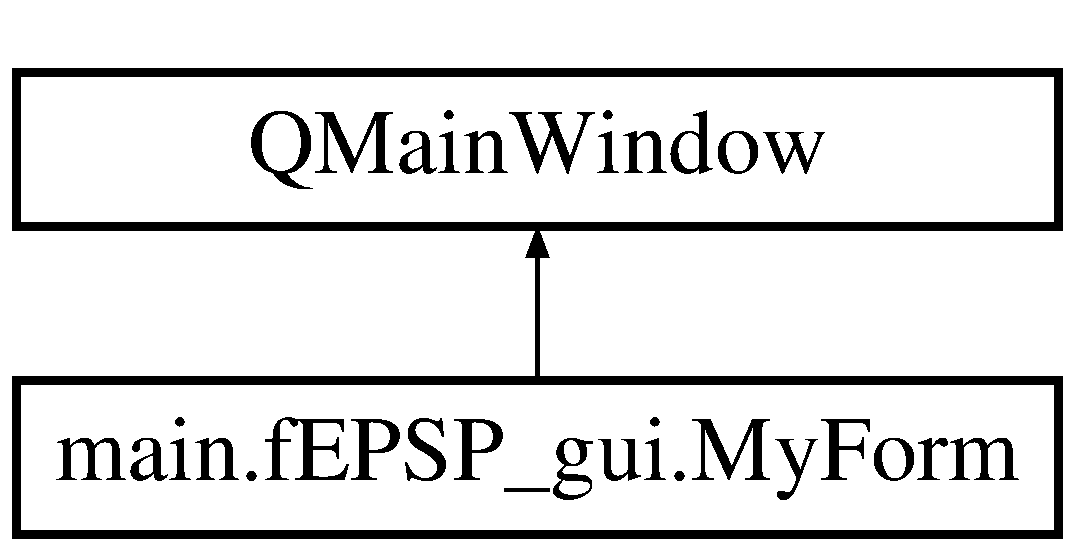
\includegraphics[height=2.000000cm]{classmain_1_1f_e_p_s_p__gui_1_1_my_form}
\end{center}
\end{figure}
\subsection*{Public Member Functions}
\begin{DoxyCompactItemize}
\item 
\hypertarget{classmain_1_1f_e_p_s_p__gui_1_1_my_form_a4a6670ae930e5066b29bb371a8d64ee1}{def {\bfseries \-\_\-\-\_\-init\-\_\-\-\_\-}}\label{classmain_1_1f_e_p_s_p__gui_1_1_my_form_a4a6670ae930e5066b29bb371a8d64ee1}

\item 
\hypertarget{classmain_1_1f_e_p_s_p__gui_1_1_my_form_a24f53a56a099522278fed7f8dadf3331}{def {\bfseries rm\-Db\-Config}}\label{classmain_1_1f_e_p_s_p__gui_1_1_my_form_a24f53a56a099522278fed7f8dadf3331}

\item 
\hypertarget{classmain_1_1f_e_p_s_p__gui_1_1_my_form_a229b335236690eaba3d1eba760f262e2}{def {\bfseries mk\-Db\-Config}}\label{classmain_1_1f_e_p_s_p__gui_1_1_my_form_a229b335236690eaba3d1eba760f262e2}

\item 
\hypertarget{classmain_1_1f_e_p_s_p__gui_1_1_my_form_a2ee046e789a670744373085ef75e3b0b}{def {\bfseries load\-Config}}\label{classmain_1_1f_e_p_s_p__gui_1_1_my_form_a2ee046e789a670744373085ef75e3b0b}

\item 
\hypertarget{classmain_1_1f_e_p_s_p__gui_1_1_my_form_adae67113d3ba9f7e84eda40223376aea}{def {\bfseries f\-E\-P\-S\-P\-\_\-start}}\label{classmain_1_1f_e_p_s_p__gui_1_1_my_form_adae67113d3ba9f7e84eda40223376aea}

\item 
\hypertarget{classmain_1_1f_e_p_s_p__gui_1_1_my_form_a42e06a0d58df1b05811ff6fea35fc8ee}{def {\bfseries show\-\_\-path}}\label{classmain_1_1f_e_p_s_p__gui_1_1_my_form_a42e06a0d58df1b05811ff6fea35fc8ee}

\item 
\hypertarget{classmain_1_1f_e_p_s_p__gui_1_1_my_form_a1a87d83b94e6106053b21d618bb135de}{def {\bfseries path\-Up}}\label{classmain_1_1f_e_p_s_p__gui_1_1_my_form_a1a87d83b94e6106053b21d618bb135de}

\item 
\hypertarget{classmain_1_1f_e_p_s_p__gui_1_1_my_form_acd5111f1804d271f3c47688a645fd184}{def {\bfseries source\-List\-Clicked}}\label{classmain_1_1f_e_p_s_p__gui_1_1_my_form_acd5111f1804d271f3c47688a645fd184}

\item 
\hypertarget{classmain_1_1f_e_p_s_p__gui_1_1_my_form_a1be8df73e677e9d8ad8be13d05aa122b}{def {\bfseries get\-Names}}\label{classmain_1_1f_e_p_s_p__gui_1_1_my_form_a1be8df73e677e9d8ad8be13d05aa122b}

\item 
\hypertarget{classmain_1_1f_e_p_s_p__gui_1_1_my_form_ab03d7483e0d4afd4aba2ee4b850b4bc5}{def {\bfseries get\-Export}}\label{classmain_1_1f_e_p_s_p__gui_1_1_my_form_ab03d7483e0d4afd4aba2ee4b850b4bc5}

\item 
\hypertarget{classmain_1_1f_e_p_s_p__gui_1_1_my_form_ac15bc24610a18bf7d8bfacefbb502d63}{def {\bfseries exp\-Name\-Update}}\label{classmain_1_1f_e_p_s_p__gui_1_1_my_form_ac15bc24610a18bf7d8bfacefbb502d63}

\item 
\hypertarget{classmain_1_1f_e_p_s_p__gui_1_1_my_form_adc657b6540d09df6d53c87c9fa85c158}{def {\bfseries export\-File\-Name\-Update}}\label{classmain_1_1f_e_p_s_p__gui_1_1_my_form_adc657b6540d09df6d53c87c9fa85c158}

\item 
\hypertarget{classmain_1_1f_e_p_s_p__gui_1_1_my_form_a226787f7ba26d922cbc6c1afdabda2d2}{def {\bfseries export}}\label{classmain_1_1f_e_p_s_p__gui_1_1_my_form_a226787f7ba26d922cbc6c1afdabda2d2}

\end{DoxyCompactItemize}
\subsection*{Public Attributes}
\begin{DoxyCompactItemize}
\item 
\hypertarget{classmain_1_1f_e_p_s_p__gui_1_1_my_form_ae000576874bd1884d94977df1d4fe0fc}{{\bfseries ui}}\label{classmain_1_1f_e_p_s_p__gui_1_1_my_form_ae000576874bd1884d94977df1d4fe0fc}

\item 
\hypertarget{classmain_1_1f_e_p_s_p__gui_1_1_my_form_abbce31a8ac2252192befed1d36459394}{{\bfseries db}}\label{classmain_1_1f_e_p_s_p__gui_1_1_my_form_abbce31a8ac2252192befed1d36459394}

\item 
\hypertarget{classmain_1_1f_e_p_s_p__gui_1_1_my_form_a74b5f9410d5c3a4e49323dd1102119e3}{{\bfseries fsmodel}}\label{classmain_1_1f_e_p_s_p__gui_1_1_my_form_a74b5f9410d5c3a4e49323dd1102119e3}

\item 
\hypertarget{classmain_1_1f_e_p_s_p__gui_1_1_my_form_a642549daead2b7fe2c3838e2f4afb40d}{{\bfseries stmodel}}\label{classmain_1_1f_e_p_s_p__gui_1_1_my_form_a642549daead2b7fe2c3838e2f4afb40d}

\item 
\hypertarget{classmain_1_1f_e_p_s_p__gui_1_1_my_form_a4995db7c3a759b091ad478e3ea3e3be4}{{\bfseries root\-\_\-index}}\label{classmain_1_1f_e_p_s_p__gui_1_1_my_form_a4995db7c3a759b091ad478e3ea3e3be4}

\item 
\hypertarget{classmain_1_1f_e_p_s_p__gui_1_1_my_form_a102cc9cd40067408a2c72b7badf9bbf5}{{\bfseries exp\-Names}}\label{classmain_1_1f_e_p_s_p__gui_1_1_my_form_a102cc9cd40067408a2c72b7badf9bbf5}

\end{DoxyCompactItemize}


\subsection{Detailed Description}


Definition at line 14 of file f\-E\-P\-S\-P\-\_\-gui.\-py.



The documentation for this class was generated from the following file\-:\begin{DoxyCompactItemize}
\item 
/home/pilat/git/f\-E\-P\-S\-P-\/analyser\-\_\-new/main/f\-E\-P\-S\-P\-\_\-gui.\-py\end{DoxyCompactItemize}

\hypertarget{classmain_1_1db_access__lib_1_1_mysql__writer}{\section{main.\-db\-Access\-\_\-lib.\-Mysql\-\_\-writer Class Reference}
\label{classmain_1_1db_access__lib_1_1_mysql__writer}\index{main.\-db\-Access\-\_\-lib.\-Mysql\-\_\-writer@{main.\-db\-Access\-\_\-lib.\-Mysql\-\_\-writer}}
}
\subsection*{Public Member Functions}
\begin{DoxyCompactItemize}
\item 
\hypertarget{classmain_1_1db_access__lib_1_1_mysql__writer_ac7ef0b7c42e9015bcbde4d1850bba2bf}{def {\bfseries \-\_\-\-\_\-init\-\_\-\-\_\-}}\label{classmain_1_1db_access__lib_1_1_mysql__writer_ac7ef0b7c42e9015bcbde4d1850bba2bf}

\item 
\hypertarget{classmain_1_1db_access__lib_1_1_mysql__writer_a6b006b96deff3431abe2659bdb2ac439}{def {\bfseries tag\-Writer}}\label{classmain_1_1db_access__lib_1_1_mysql__writer_a6b006b96deff3431abe2659bdb2ac439}

\item 
\hypertarget{classmain_1_1db_access__lib_1_1_mysql__writer_a7c61f6a4987eca3fc114750658273a9f}{def {\bfseries tag\-Check}}\label{classmain_1_1db_access__lib_1_1_mysql__writer_a7c61f6a4987eca3fc114750658273a9f}

\item 
\hypertarget{classmain_1_1db_access__lib_1_1_mysql__writer_a326a5ac025c850077cf7a50f1c0d87e8}{def {\bfseries variables\-\_\-global}}\label{classmain_1_1db_access__lib_1_1_mysql__writer_a326a5ac025c850077cf7a50f1c0d87e8}

\item 
\hypertarget{classmain_1_1db_access__lib_1_1_mysql__writer_af6c4d1ee9f32b1a8332770a9f0410669}{def {\bfseries variables\-\_\-local}}\label{classmain_1_1db_access__lib_1_1_mysql__writer_af6c4d1ee9f32b1a8332770a9f0410669}

\item 
\hypertarget{classmain_1_1db_access__lib_1_1_mysql__writer_ade5de279756f6f660fe54db385e2fe27}{def {\bfseries db\-Connect}}\label{classmain_1_1db_access__lib_1_1_mysql__writer_ade5de279756f6f660fe54db385e2fe27}

\item 
\hypertarget{classmain_1_1db_access__lib_1_1_mysql__writer_aac403a3701e71603a845b7dece7a069f}{def {\bfseries db\-Write\-Experiment}}\label{classmain_1_1db_access__lib_1_1_mysql__writer_aac403a3701e71603a845b7dece7a069f}

\item 
\hypertarget{classmain_1_1db_access__lib_1_1_mysql__writer_a0cb738adec1207afde820447cdbd426c}{def {\bfseries db\-Write\-Record}}\label{classmain_1_1db_access__lib_1_1_mysql__writer_a0cb738adec1207afde820447cdbd426c}

\item 
\hypertarget{classmain_1_1db_access__lib_1_1_mysql__writer_a288181e3dc9cd10bffc201461b881f79}{def {\bfseries find\-Tags}}\label{classmain_1_1db_access__lib_1_1_mysql__writer_a288181e3dc9cd10bffc201461b881f79}

\item 
\hypertarget{classmain_1_1db_access__lib_1_1_mysql__writer_af39fd76d137cea0d22430184eafb6d5d}{def {\bfseries get\-Exp\-Names}}\label{classmain_1_1db_access__lib_1_1_mysql__writer_af39fd76d137cea0d22430184eafb6d5d}

\item 
\hypertarget{classmain_1_1db_access__lib_1_1_mysql__writer_a77732efa2af097674071384f482167b8}{def {\bfseries get\-Data\-To\-Export}}\label{classmain_1_1db_access__lib_1_1_mysql__writer_a77732efa2af097674071384f482167b8}

\item 
\hypertarget{classmain_1_1db_access__lib_1_1_mysql__writer_a3682bacec440542255c181d434e9568a}{def {\bfseries db\-Write\-Record\-Tags}}\label{classmain_1_1db_access__lib_1_1_mysql__writer_a3682bacec440542255c181d434e9568a}

\item 
\hypertarget{classmain_1_1db_access__lib_1_1_mysql__writer_abd077f389125c061b7f8931cf12cbae8}{def {\bfseries db\-Write\-Response}}\label{classmain_1_1db_access__lib_1_1_mysql__writer_abd077f389125c061b7f8931cf12cbae8}

\item 
\hypertarget{classmain_1_1db_access__lib_1_1_mysql__writer_ab5d8f6dd46cdf98b885b13d81243b05c}{def {\bfseries db\-Write\-Number\-Of\-Responses}}\label{classmain_1_1db_access__lib_1_1_mysql__writer_ab5d8f6dd46cdf98b885b13d81243b05c}

\item 
\hypertarget{classmain_1_1db_access__lib_1_1_mysql__writer_ad81cf7d290a00037d1c940966f0ac143}{def {\bfseries db\-Write\-Signal\-Properties}}\label{classmain_1_1db_access__lib_1_1_mysql__writer_ad81cf7d290a00037d1c940966f0ac143}

\item 
\hypertarget{classmain_1_1db_access__lib_1_1_mysql__writer_a82b1f0bdc82b53949c0bf22b7517a9fd}{def {\bfseries db\-Write\-Error}}\label{classmain_1_1db_access__lib_1_1_mysql__writer_a82b1f0bdc82b53949c0bf22b7517a9fd}

\item 
\hypertarget{classmain_1_1db_access__lib_1_1_mysql__writer_a3cc119685849462b059f2ed2d81c35b3}{def {\bfseries db\-Write\-Spike}}\label{classmain_1_1db_access__lib_1_1_mysql__writer_a3cc119685849462b059f2ed2d81c35b3}

\item 
\hypertarget{classmain_1_1db_access__lib_1_1_mysql__writer_a9c472f99fe6b1204e933e56fb57cd3d2}{def {\bfseries db\-Disconnect}}\label{classmain_1_1db_access__lib_1_1_mysql__writer_a9c472f99fe6b1204e933e56fb57cd3d2}

\item 
\hypertarget{classmain_1_1db_access__lib_1_1_mysql__writer_a18378c9ed05f826eaed3a765054fce77}{def {\bfseries db\-Write\-Stim}}\label{classmain_1_1db_access__lib_1_1_mysql__writer_a18378c9ed05f826eaed3a765054fce77}

\end{DoxyCompactItemize}
\subsection*{Public Attributes}
\begin{DoxyCompactItemize}
\item 
\hypertarget{classmain_1_1db_access__lib_1_1_mysql__writer_a76dd160634eec9223ff965cbaa09dae9}{{\bfseries file\-Path}}\label{classmain_1_1db_access__lib_1_1_mysql__writer_a76dd160634eec9223ff965cbaa09dae9}

\item 
\hypertarget{classmain_1_1db_access__lib_1_1_mysql__writer_ab1ad1b5d7ced6bcc4ff6f8b0c28d06cb}{{\bfseries tag\-String}}\label{classmain_1_1db_access__lib_1_1_mysql__writer_ab1ad1b5d7ced6bcc4ff6f8b0c28d06cb}

\item 
\hypertarget{classmain_1_1db_access__lib_1_1_mysql__writer_a7505c6129b4e7f684bcbdf982069e7a0}{{\bfseries r\-Tag\-Dict}}\label{classmain_1_1db_access__lib_1_1_mysql__writer_a7505c6129b4e7f684bcbdf982069e7a0}

\item 
\hypertarget{classmain_1_1db_access__lib_1_1_mysql__writer_a33f2e83b06202cf5ec8130b1d5cac2d2}{{\bfseries r\-Tag\-Mask}}\label{classmain_1_1db_access__lib_1_1_mysql__writer_a33f2e83b06202cf5ec8130b1d5cac2d2}

\item 
\hypertarget{classmain_1_1db_access__lib_1_1_mysql__writer_a716c3922a84e28b1aab64d6cfcfb9c17}{{\bfseries koef}}\label{classmain_1_1db_access__lib_1_1_mysql__writer_a716c3922a84e28b1aab64d6cfcfb9c17}

\item 
\hypertarget{classmain_1_1db_access__lib_1_1_mysql__writer_a9d74f3c29da544fda07991596ad0525d}{{\bfseries db\-Server\-Ip}}\label{classmain_1_1db_access__lib_1_1_mysql__writer_a9d74f3c29da544fda07991596ad0525d}

\item 
\hypertarget{classmain_1_1db_access__lib_1_1_mysql__writer_a913edf72906fbedb9ce50fbc333ed64a}{{\bfseries user\-Name}}\label{classmain_1_1db_access__lib_1_1_mysql__writer_a913edf72906fbedb9ce50fbc333ed64a}

\item 
\hypertarget{classmain_1_1db_access__lib_1_1_mysql__writer_ac694836e86f8909b19a64b6a0fcad63c}{{\bfseries user\-Password}}\label{classmain_1_1db_access__lib_1_1_mysql__writer_ac694836e86f8909b19a64b6a0fcad63c}

\item 
\hypertarget{classmain_1_1db_access__lib_1_1_mysql__writer_a02c7f19727bacca099177c68b75c86be}{{\bfseries db\-Name}}\label{classmain_1_1db_access__lib_1_1_mysql__writer_a02c7f19727bacca099177c68b75c86be}

\item 
\hypertarget{classmain_1_1db_access__lib_1_1_mysql__writer_a0b8b6cf41c30b507da7eb7ce6e2dbcbf}{{\bfseries date}}\label{classmain_1_1db_access__lib_1_1_mysql__writer_a0b8b6cf41c30b507da7eb7ce6e2dbcbf}

\item 
\hypertarget{classmain_1_1db_access__lib_1_1_mysql__writer_a28bcc05f6a8b330a676fbbc66a1fb9b2}{{\bfseries respons\-Number}}\label{classmain_1_1db_access__lib_1_1_mysql__writer_a28bcc05f6a8b330a676fbbc66a1fb9b2}

\item 
\hypertarget{classmain_1_1db_access__lib_1_1_mysql__writer_ad8a4edcae9c7b561215c8cae17344e66}{{\bfseries numberofspikes}}\label{classmain_1_1db_access__lib_1_1_mysql__writer_ad8a4edcae9c7b561215c8cae17344e66}

\item 
\hypertarget{classmain_1_1db_access__lib_1_1_mysql__writer_a1e7a91a2786f2cf96edcbf3dcee6f9af}{{\bfseries responslength}}\label{classmain_1_1db_access__lib_1_1_mysql__writer_a1e7a91a2786f2cf96edcbf3dcee6f9af}

\item 
\hypertarget{classmain_1_1db_access__lib_1_1_mysql__writer_a4752389a714ad5c4fc67c711a3839108}{{\bfseries ampl}}\label{classmain_1_1db_access__lib_1_1_mysql__writer_a4752389a714ad5c4fc67c711a3839108}

\item 
\hypertarget{classmain_1_1db_access__lib_1_1_mysql__writer_ac4665b948d3acfe1f985bd441f58e137}{{\bfseries number}}\label{classmain_1_1db_access__lib_1_1_mysql__writer_ac4665b948d3acfe1f985bd441f58e137}

\item 
\hypertarget{classmain_1_1db_access__lib_1_1_mysql__writer_aca06ba72c02805f1675c4b8ce6e247cc}{{\bfseries conn}}\label{classmain_1_1db_access__lib_1_1_mysql__writer_aca06ba72c02805f1675c4b8ce6e247cc}

\item 
\hypertarget{classmain_1_1db_access__lib_1_1_mysql__writer_ac1578364e6acd9a713d1e66acfae6880}{{\bfseries id\-Experiment}}\label{classmain_1_1db_access__lib_1_1_mysql__writer_ac1578364e6acd9a713d1e66acfae6880}

\item 
\hypertarget{classmain_1_1db_access__lib_1_1_mysql__writer_a9147d2e8114caf4d284a490cc14696e0}{{\bfseries id\-Record}}\label{classmain_1_1db_access__lib_1_1_mysql__writer_a9147d2e8114caf4d284a490cc14696e0}

\end{DoxyCompactItemize}


\subsection{Detailed Description}


Definition at line 13 of file db\-Access\-\_\-lib.\-py.



The documentation for this class was generated from the following file\-:\begin{DoxyCompactItemize}
\item 
/home/pilat/git/f\-E\-P\-S\-P-\/analyser\-\_\-new/main/db\-Access\-\_\-lib.\-py\end{DoxyCompactItemize}

\hypertarget{classmain_1_1objects__lib_1_1_response}{\section{main.\-objects\-\_\-lib.\-Response Class Reference}
\label{classmain_1_1objects__lib_1_1_response}\index{main.\-objects\-\_\-lib.\-Response@{main.\-objects\-\_\-lib.\-Response}}
}
\subsection*{Public Member Functions}
\begin{DoxyCompactItemize}
\item 
\hypertarget{classmain_1_1objects__lib_1_1_response_ac9544849f6abfe64908561caa6387280}{def {\bfseries \-\_\-\-\_\-init\-\_\-\-\_\-}}\label{classmain_1_1objects__lib_1_1_response_ac9544849f6abfe64908561caa6387280}

\end{DoxyCompactItemize}
\subsection*{Public Attributes}
\begin{DoxyCompactItemize}
\item 
\hypertarget{classmain_1_1objects__lib_1_1_response_ab6f23603a45be2336b3d1c31662b44fc}{{\bfseries epsp\-Front}}\label{classmain_1_1objects__lib_1_1_response_ab6f23603a45be2336b3d1c31662b44fc}

\item 
\hypertarget{classmain_1_1objects__lib_1_1_response_a28803f03692a76cbc8cfacb0cbabb82f}{{\bfseries epsp\-Back}}\label{classmain_1_1objects__lib_1_1_response_a28803f03692a76cbc8cfacb0cbabb82f}

\item 
\hypertarget{classmain_1_1objects__lib_1_1_response_ae26070df8764b6498c2e80d805fbec9f}{{\bfseries epsp\-Epilept\-Std}}\label{classmain_1_1objects__lib_1_1_response_ae26070df8764b6498c2e80d805fbec9f}

\item 
\hypertarget{classmain_1_1objects__lib_1_1_response_a62727276da5815103a4d337146c111ca}{{\bfseries fibre}}\label{classmain_1_1objects__lib_1_1_response_a62727276da5815103a4d337146c111ca}

\item 
\hypertarget{classmain_1_1objects__lib_1_1_response_a8da58ce9eaa0a2abb13f228e722eeb54}{{\bfseries epsp\-Area}}\label{classmain_1_1objects__lib_1_1_response_a8da58ce9eaa0a2abb13f228e722eeb54}

\end{DoxyCompactItemize}


\subsection{Detailed Description}


Definition at line 33 of file objects\-\_\-lib.\-py.



The documentation for this class was generated from the following file\-:\begin{DoxyCompactItemize}
\item 
/home/pilat/git/f\-E\-P\-S\-P-\/analyser\-\_\-new/main/objects\-\_\-lib.\-py\end{DoxyCompactItemize}

\hypertarget{classmain_1_1objects__lib_1_1_spike}{\section{main.\-objects\-\_\-lib.\-Spike Class Reference}
\label{classmain_1_1objects__lib_1_1_spike}\index{main.\-objects\-\_\-lib.\-Spike@{main.\-objects\-\_\-lib.\-Spike}}
}
\subsection*{Public Member Functions}
\begin{DoxyCompactItemize}
\item 
\hypertarget{classmain_1_1objects__lib_1_1_spike_adb235c1830eaaf58ee905fd6bca00914}{def {\bfseries \-\_\-\-\_\-init\-\_\-\-\_\-}}\label{classmain_1_1objects__lib_1_1_spike_adb235c1830eaaf58ee905fd6bca00914}

\end{DoxyCompactItemize}
\subsection*{Public Attributes}
\begin{DoxyCompactItemize}
\item 
\hypertarget{classmain_1_1objects__lib_1_1_spike_aa7b0b6d3a467e3d15c89aa698ae7950a}{{\bfseries response\-Number}}\label{classmain_1_1objects__lib_1_1_spike_aa7b0b6d3a467e3d15c89aa698ae7950a}

\item 
\hypertarget{classmain_1_1objects__lib_1_1_spike_a3753114da2b9d1f3980d8bde25328ea8}{{\bfseries response\-Start}}\label{classmain_1_1objects__lib_1_1_spike_a3753114da2b9d1f3980d8bde25328ea8}

\item 
\hypertarget{classmain_1_1objects__lib_1_1_spike_aef4d9a9e774865d11e1d0aa58869754e}{{\bfseries response\-End}}\label{classmain_1_1objects__lib_1_1_spike_aef4d9a9e774865d11e1d0aa58869754e}

\item 
\hypertarget{classmain_1_1objects__lib_1_1_spike_af17a4ee0a5656cc1d5232b93bd265a53}{{\bfseries spike\-Number}}\label{classmain_1_1objects__lib_1_1_spike_af17a4ee0a5656cc1d5232b93bd265a53}

\item 
\hypertarget{classmain_1_1objects__lib_1_1_spike_a7962eec37d2d7d6b95bfd7206c5f727a}{{\bfseries all\-Spikes}}\label{classmain_1_1objects__lib_1_1_spike_a7962eec37d2d7d6b95bfd7206c5f727a}

\item 
\hypertarget{classmain_1_1objects__lib_1_1_spike_a5b73e596402a4d6217fc362ca04b3c6d}{{\bfseries spike\-Max1}}\label{classmain_1_1objects__lib_1_1_spike_a5b73e596402a4d6217fc362ca04b3c6d}

\item 
\hypertarget{classmain_1_1objects__lib_1_1_spike_aa157731db95ae300b323eb8d90bca212}{{\bfseries spike\-Min}}\label{classmain_1_1objects__lib_1_1_spike_aa157731db95ae300b323eb8d90bca212}

\item 
\hypertarget{classmain_1_1objects__lib_1_1_spike_a6c1dd24723e3145ee83fd375ed8b48ab}{{\bfseries spike\-Max2}}\label{classmain_1_1objects__lib_1_1_spike_a6c1dd24723e3145ee83fd375ed8b48ab}

\item 
\hypertarget{classmain_1_1objects__lib_1_1_spike_a5cf989abf643096118c6bbc1ddd01e15}{{\bfseries spike\-Ampl}}\label{classmain_1_1objects__lib_1_1_spike_a5cf989abf643096118c6bbc1ddd01e15}

\item 
\hypertarget{classmain_1_1objects__lib_1_1_spike_a09c9c562b159df3d0ceb13f9b142181e}{{\bfseries frequency}}\label{classmain_1_1objects__lib_1_1_spike_a09c9c562b159df3d0ceb13f9b142181e}

\item 
\hypertarget{classmain_1_1objects__lib_1_1_spike_a3d57385e2b11d90fd6a695cd8dbb1677}{{\bfseries spike\-Length}}\label{classmain_1_1objects__lib_1_1_spike_a3d57385e2b11d90fd6a695cd8dbb1677}

\item 
\hypertarget{classmain_1_1objects__lib_1_1_spike_a983ccac2ae11a2183a15454af69e2d3e}{{\bfseries spike\-Frequency}}\label{classmain_1_1objects__lib_1_1_spike_a983ccac2ae11a2183a15454af69e2d3e}

\item 
\hypertarget{classmain_1_1objects__lib_1_1_spike_aadd26806bec52b1c2e02c692d3e91c8b}{{\bfseries spike\-Front}}\label{classmain_1_1objects__lib_1_1_spike_aadd26806bec52b1c2e02c692d3e91c8b}

\item 
\hypertarget{classmain_1_1objects__lib_1_1_spike_afaebdfae2f1b2b6cb6d4a62bd80e71dc}{{\bfseries spike\-Back}}\label{classmain_1_1objects__lib_1_1_spike_afaebdfae2f1b2b6cb6d4a62bd80e71dc}

\item 
\hypertarget{classmain_1_1objects__lib_1_1_spike_ab2a9e98bbc1d75d3bb3b6a51163ac3a0}{{\bfseries area}}\label{classmain_1_1objects__lib_1_1_spike_ab2a9e98bbc1d75d3bb3b6a51163ac3a0}

\item 
\hypertarget{classmain_1_1objects__lib_1_1_spike_a3fc22aa18afca14b858789e016902e25}{{\bfseries fibre}}\label{classmain_1_1objects__lib_1_1_spike_a3fc22aa18afca14b858789e016902e25}

\item 
\hypertarget{classmain_1_1objects__lib_1_1_spike_a32fbff292f206f38ed15497a9174367e}{{\bfseries manual}}\label{classmain_1_1objects__lib_1_1_spike_a32fbff292f206f38ed15497a9174367e}

\item 
\hypertarget{classmain_1_1objects__lib_1_1_spike_a12adbb3297e0240f54ddb6e6fe8dca5a}{{\bfseries spike\-Delay}}\label{classmain_1_1objects__lib_1_1_spike_a12adbb3297e0240f54ddb6e6fe8dca5a}

\end{DoxyCompactItemize}


\subsection{Detailed Description}


Definition at line 9 of file objects\-\_\-lib.\-py.



The documentation for this class was generated from the following file\-:\begin{DoxyCompactItemize}
\item 
/home/pilat/git/f\-E\-P\-S\-P-\/analyser\-\_\-new/main/objects\-\_\-lib.\-py\end{DoxyCompactItemize}

\hypertarget{classmain_1_1simple_1_1_ui___main_window}{\section{main.\-simple.\-Ui\-\_\-\-Main\-Window Class Reference}
\label{classmain_1_1simple_1_1_ui___main_window}\index{main.\-simple.\-Ui\-\_\-\-Main\-Window@{main.\-simple.\-Ui\-\_\-\-Main\-Window}}
}
Inheritance diagram for main.\-simple.\-Ui\-\_\-\-Main\-Window\-:\begin{figure}[H]
\begin{center}
\leavevmode
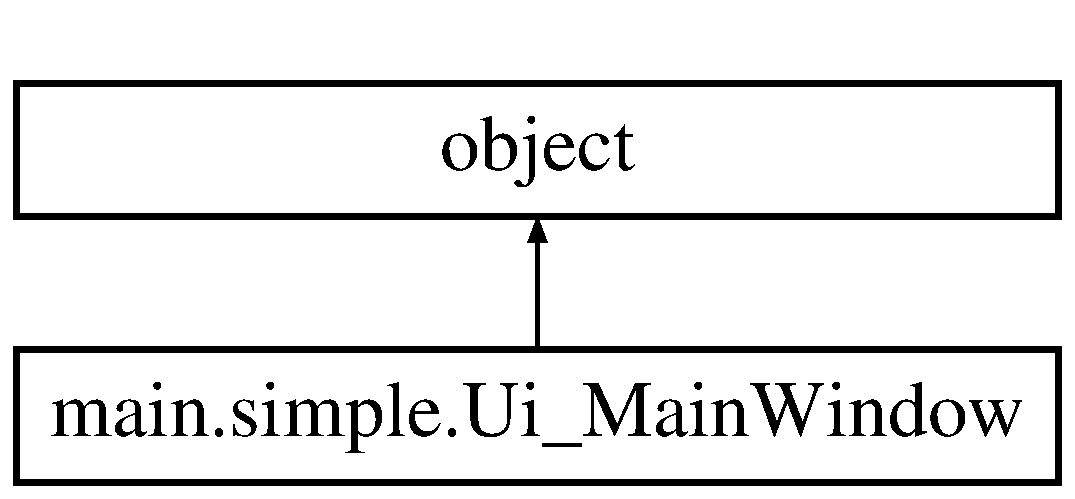
\includegraphics[height=2.000000cm]{classmain_1_1simple_1_1_ui___main_window}
\end{center}
\end{figure}
\subsection*{Public Member Functions}
\begin{DoxyCompactItemize}
\item 
\hypertarget{classmain_1_1simple_1_1_ui___main_window_a9fc239b6f0036e1361503ecfcab4b2c0}{def {\bfseries setup\-Ui}}\label{classmain_1_1simple_1_1_ui___main_window_a9fc239b6f0036e1361503ecfcab4b2c0}

\item 
\hypertarget{classmain_1_1simple_1_1_ui___main_window_a948a84517b1c5315e44efd062573fb75}{def {\bfseries retranslate\-Ui}}\label{classmain_1_1simple_1_1_ui___main_window_a948a84517b1c5315e44efd062573fb75}

\end{DoxyCompactItemize}
\subsection*{Public Attributes}
\begin{DoxyCompactItemize}
\item 
\hypertarget{classmain_1_1simple_1_1_ui___main_window_a245234845d98495227b04a1839278527}{{\bfseries centralwidget}}\label{classmain_1_1simple_1_1_ui___main_window_a245234845d98495227b04a1839278527}

\item 
\hypertarget{classmain_1_1simple_1_1_ui___main_window_a66ffc87503c0deea9bcd9047efbc9b9d}{{\bfseries source\-List}}\label{classmain_1_1simple_1_1_ui___main_window_a66ffc87503c0deea9bcd9047efbc9b9d}

\item 
\hypertarget{classmain_1_1simple_1_1_ui___main_window_a7cf0d15838599b220352ed7e9abe6141}{{\bfseries path\-Line}}\label{classmain_1_1simple_1_1_ui___main_window_a7cf0d15838599b220352ed7e9abe6141}

\item 
\hypertarget{classmain_1_1simple_1_1_ui___main_window_a712292fe3624a94966557535847c68ae}{{\bfseries path\-Label}}\label{classmain_1_1simple_1_1_ui___main_window_a712292fe3624a94966557535847c68ae}

\item 
\hypertarget{classmain_1_1simple_1_1_ui___main_window_a5c2835fbb3bb327f39265aaf77f0dff1}{{\bfseries exit\-Button}}\label{classmain_1_1simple_1_1_ui___main_window_a5c2835fbb3bb327f39265aaf77f0dff1}

\item 
\hypertarget{classmain_1_1simple_1_1_ui___main_window_a7ce19628ad86388a1ba09e7d3ca453c4}{{\bfseries up\-Button}}\label{classmain_1_1simple_1_1_ui___main_window_a7ce19628ad86388a1ba09e7d3ca453c4}

\item 
\hypertarget{classmain_1_1simple_1_1_ui___main_window_a3b85e05cf1ba2d185e8230160d0351f3}{{\bfseries text\-Browser}}\label{classmain_1_1simple_1_1_ui___main_window_a3b85e05cf1ba2d185e8230160d0351f3}

\item 
\hypertarget{classmain_1_1simple_1_1_ui___main_window_a9171604d93428f1f0b965eb8d4af3495}{{\bfseries tab\-Widget}}\label{classmain_1_1simple_1_1_ui___main_window_a9171604d93428f1f0b965eb8d4af3495}

\item 
\hypertarget{classmain_1_1simple_1_1_ui___main_window_af98965c1326dd50ac2076ff3acb84946}{{\bfseries f\-E\-P\-S\-Panalyser}}\label{classmain_1_1simple_1_1_ui___main_window_af98965c1326dd50ac2076ff3acb84946}

\item 
\hypertarget{classmain_1_1simple_1_1_ui___main_window_a5cbd1af3d0533b7c85c702b4be3871b4}{{\bfseries vertical\-Layout\-Widget\-\_\-2}}\label{classmain_1_1simple_1_1_ui___main_window_a5cbd1af3d0533b7c85c702b4be3871b4}

\item 
\hypertarget{classmain_1_1simple_1_1_ui___main_window_a2aee356d8f916d42032dd1b09b732721}{{\bfseries vertical\-Layout\-\_\-2}}\label{classmain_1_1simple_1_1_ui___main_window_a2aee356d8f916d42032dd1b09b732721}

\item 
\hypertarget{classmain_1_1simple_1_1_ui___main_window_a755175861056f1a926b0b733decad7b0}{{\bfseries grid\-Layout\-\_\-2}}\label{classmain_1_1simple_1_1_ui___main_window_a755175861056f1a926b0b733decad7b0}

\item 
\hypertarget{classmain_1_1simple_1_1_ui___main_window_acde8b64cac7b97a0117ac8824085f68d}{{\bfseries frequency\-\_\-line}}\label{classmain_1_1simple_1_1_ui___main_window_acde8b64cac7b97a0117ac8824085f68d}

\item 
\hypertarget{classmain_1_1simple_1_1_ui___main_window_aa24132fe7d98bb9f9307d1e50dc07825}{{\bfseries substance\-\_\-line}}\label{classmain_1_1simple_1_1_ui___main_window_aa24132fe7d98bb9f9307d1e50dc07825}

\item 
\hypertarget{classmain_1_1simple_1_1_ui___main_window_ac3fef1e197a482a8913318e2b71715f2}{{\bfseries label\-\_\-3}}\label{classmain_1_1simple_1_1_ui___main_window_ac3fef1e197a482a8913318e2b71715f2}

\item 
\hypertarget{classmain_1_1simple_1_1_ui___main_window_af20a8a198df977a1622621c1edc8776e}{{\bfseries label\-\_\-2}}\label{classmain_1_1simple_1_1_ui___main_window_af20a8a198df977a1622621c1edc8776e}

\item 
\hypertarget{classmain_1_1simple_1_1_ui___main_window_ade69f101c10e3b5dbb6b45ddbaef9a4c}{{\bfseries horizontal\-Layout}}\label{classmain_1_1simple_1_1_ui___main_window_ade69f101c10e3b5dbb6b45ddbaef9a4c}

\item 
\hypertarget{classmain_1_1simple_1_1_ui___main_window_a72cb019bda0145bd2bf2bdd9e0c33e1b}{{\bfseries vertical\-Layout}}\label{classmain_1_1simple_1_1_ui___main_window_a72cb019bda0145bd2bf2bdd9e0c33e1b}

\item 
\hypertarget{classmain_1_1simple_1_1_ui___main_window_a97a7a5810ae6fa86aae96db3f9369d86}{{\bfseries database\-\_\-check\-Box}}\label{classmain_1_1simple_1_1_ui___main_window_a97a7a5810ae6fa86aae96db3f9369d86}

\item 
\hypertarget{classmain_1_1simple_1_1_ui___main_window_afdb49043ad533631200803acdcfb3355}{{\bfseries debug\-Box}}\label{classmain_1_1simple_1_1_ui___main_window_afdb49043ad533631200803acdcfb3355}

\item 
\hypertarget{classmain_1_1simple_1_1_ui___main_window_ab33371ebc5acdeac3b685f1ca1d664b2}{{\bfseries manual\-Fibre\-Search\-Box}}\label{classmain_1_1simple_1_1_ui___main_window_ab33371ebc5acdeac3b685f1ca1d664b2}

\item 
\hypertarget{classmain_1_1simple_1_1_ui___main_window_acc095cd8de28521395aff46280de8d47}{{\bfseries horizontal\-Layout\-\_\-5}}\label{classmain_1_1simple_1_1_ui___main_window_acc095cd8de28521395aff46280de8d47}

\item 
\hypertarget{classmain_1_1simple_1_1_ui___main_window_aa1a079ad2af073612b72dda3b14075b5}{{\bfseries smooth\-Box}}\label{classmain_1_1simple_1_1_ui___main_window_aa1a079ad2af073612b72dda3b14075b5}

\item 
\hypertarget{classmain_1_1simple_1_1_ui___main_window_a1f86aa2ed49f4d6884277288f27d4a4f}{{\bfseries label\-\_\-6}}\label{classmain_1_1simple_1_1_ui___main_window_a1f86aa2ed49f4d6884277288f27d4a4f}

\item 
\hypertarget{classmain_1_1simple_1_1_ui___main_window_a45a1b36451508bf15699f85a7b82dda8}{{\bfseries f\-E\-P\-S\-P\-\_\-button}}\label{classmain_1_1simple_1_1_ui___main_window_a45a1b36451508bf15699f85a7b82dda8}

\item 
\hypertarget{classmain_1_1simple_1_1_ui___main_window_a570a2805012df38de66dc6e3247217df}{{\bfseries export\-Tab}}\label{classmain_1_1simple_1_1_ui___main_window_a570a2805012df38de66dc6e3247217df}

\item 
\hypertarget{classmain_1_1simple_1_1_ui___main_window_a490f41ffc0f13e6149130005b22e054a}{{\bfseries vertical\-Layout\-Widget\-\_\-3}}\label{classmain_1_1simple_1_1_ui___main_window_a490f41ffc0f13e6149130005b22e054a}

\item 
\hypertarget{classmain_1_1simple_1_1_ui___main_window_a373bfcb152cd4e4dba1f0524329230da}{{\bfseries vertical\-Layout\-\_\-3}}\label{classmain_1_1simple_1_1_ui___main_window_a373bfcb152cd4e4dba1f0524329230da}

\item 
\hypertarget{classmain_1_1simple_1_1_ui___main_window_aa10aeca355addedf102a18639c44172a}{{\bfseries label}}\label{classmain_1_1simple_1_1_ui___main_window_aa10aeca355addedf102a18639c44172a}

\item 
\hypertarget{classmain_1_1simple_1_1_ui___main_window_a7f974a71dbf467c3a81df8beb091c06d}{{\bfseries horizontal\-Layout\-\_\-2}}\label{classmain_1_1simple_1_1_ui___main_window_a7f974a71dbf467c3a81df8beb091c06d}

\item 
\hypertarget{classmain_1_1simple_1_1_ui___main_window_a71ab04a605ec9a47f130c6f35add953d}{{\bfseries export\-Exp\-Name}}\label{classmain_1_1simple_1_1_ui___main_window_a71ab04a605ec9a47f130c6f35add953d}

\item 
\hypertarget{classmain_1_1simple_1_1_ui___main_window_aea0f2d7c74ceeaaf876770a760d4b305}{{\bfseries export\-Refresh}}\label{classmain_1_1simple_1_1_ui___main_window_aea0f2d7c74ceeaaf876770a760d4b305}

\item 
\hypertarget{classmain_1_1simple_1_1_ui___main_window_abc43c58bac91708209283398a0e842f7}{{\bfseries label\-\_\-4}}\label{classmain_1_1simple_1_1_ui___main_window_abc43c58bac91708209283398a0e842f7}

\item 
\hypertarget{classmain_1_1simple_1_1_ui___main_window_a555079be3f38428557698002818f25fb}{{\bfseries export\-Spike}}\label{classmain_1_1simple_1_1_ui___main_window_a555079be3f38428557698002818f25fb}

\item 
\hypertarget{classmain_1_1simple_1_1_ui___main_window_a55243c6257135fbd2d0ea1ca9536e26c}{{\bfseries label\-\_\-5}}\label{classmain_1_1simple_1_1_ui___main_window_a55243c6257135fbd2d0ea1ca9536e26c}

\item 
\hypertarget{classmain_1_1simple_1_1_ui___main_window_a8e3fc15b55501ff223edd36000c1d030}{{\bfseries horizontal\-Layout\-\_\-4}}\label{classmain_1_1simple_1_1_ui___main_window_a8e3fc15b55501ff223edd36000c1d030}

\item 
\hypertarget{classmain_1_1simple_1_1_ui___main_window_a2fe33cc08928b5e907383c54174642f3}{{\bfseries export\-Filename}}\label{classmain_1_1simple_1_1_ui___main_window_a2fe33cc08928b5e907383c54174642f3}

\item 
\hypertarget{classmain_1_1simple_1_1_ui___main_window_a95f3b5b6cd557c9999d47c9cee72a049}{{\bfseries export\-Button}}\label{classmain_1_1simple_1_1_ui___main_window_a95f3b5b6cd557c9999d47c9cee72a049}

\item 
\hypertarget{classmain_1_1simple_1_1_ui___main_window_a37839505ae3dc36519aa87275abd6972}{{\bfseries tab\-\_\-2}}\label{classmain_1_1simple_1_1_ui___main_window_a37839505ae3dc36519aa87275abd6972}

\item 
\hypertarget{classmain_1_1simple_1_1_ui___main_window_a9214bfab7a7c8c22f7623bc8e6d084d0}{{\bfseries frame}}\label{classmain_1_1simple_1_1_ui___main_window_a9214bfab7a7c8c22f7623bc8e6d084d0}

\item 
\hypertarget{classmain_1_1simple_1_1_ui___main_window_ad1d87b2767968be16a892ec951d2bd74}{{\bfseries horizontal\-Layout\-Widget\-\_\-3}}\label{classmain_1_1simple_1_1_ui___main_window_ad1d87b2767968be16a892ec951d2bd74}

\item 
\hypertarget{classmain_1_1simple_1_1_ui___main_window_a887fd98b6e88aa8468fc3792ccf9cc91}{{\bfseries horizontal\-Layout\-\_\-3}}\label{classmain_1_1simple_1_1_ui___main_window_a887fd98b6e88aa8468fc3792ccf9cc91}

\item 
\hypertarget{classmain_1_1simple_1_1_ui___main_window_a7b7296bc74d7a59923f7f4e9d0c3ee96}{{\bfseries save\-Db\-Button}}\label{classmain_1_1simple_1_1_ui___main_window_a7b7296bc74d7a59923f7f4e9d0c3ee96}

\item 
\hypertarget{classmain_1_1simple_1_1_ui___main_window_a316ebb773f890b17a89e16f437c17066}{{\bfseries clear\-Db\-Button}}\label{classmain_1_1simple_1_1_ui___main_window_a316ebb773f890b17a89e16f437c17066}

\item 
\hypertarget{classmain_1_1simple_1_1_ui___main_window_acda8277339cfa11bff206aaea32b98d9}{{\bfseries layout\-Widget}}\label{classmain_1_1simple_1_1_ui___main_window_acda8277339cfa11bff206aaea32b98d9}

\item 
\hypertarget{classmain_1_1simple_1_1_ui___main_window_a9e9abdb9db71e49a3f33ba88a168868a}{{\bfseries grid\-Layout\-\_\-4}}\label{classmain_1_1simple_1_1_ui___main_window_a9e9abdb9db71e49a3f33ba88a168868a}

\item 
\hypertarget{classmain_1_1simple_1_1_ui___main_window_ada53a5393ac8cc7915e378a33eb8fda5}{{\bfseries label\-\_\-7}}\label{classmain_1_1simple_1_1_ui___main_window_ada53a5393ac8cc7915e378a33eb8fda5}

\item 
\hypertarget{classmain_1_1simple_1_1_ui___main_window_a67f5dd9cd15482788d04340740e758db}{{\bfseries db\-Name\-Line}}\label{classmain_1_1simple_1_1_ui___main_window_a67f5dd9cd15482788d04340740e758db}

\item 
\hypertarget{classmain_1_1simple_1_1_ui___main_window_a80a88f2f955c2490601450716e551993}{{\bfseries label\-\_\-8}}\label{classmain_1_1simple_1_1_ui___main_window_a80a88f2f955c2490601450716e551993}

\item 
\hypertarget{classmain_1_1simple_1_1_ui___main_window_ab335a6911600e03a8c764ba662c98e84}{{\bfseries db\-User\-Line}}\label{classmain_1_1simple_1_1_ui___main_window_ab335a6911600e03a8c764ba662c98e84}

\item 
\hypertarget{classmain_1_1simple_1_1_ui___main_window_ab78c7d72d37efa8dbcd0230b9064146c}{{\bfseries label\-\_\-9}}\label{classmain_1_1simple_1_1_ui___main_window_ab78c7d72d37efa8dbcd0230b9064146c}

\item 
\hypertarget{classmain_1_1simple_1_1_ui___main_window_aff1d80b5908909bcd1bb4da955608174}{{\bfseries db\-Pass\-Line}}\label{classmain_1_1simple_1_1_ui___main_window_aff1d80b5908909bcd1bb4da955608174}

\item 
\hypertarget{classmain_1_1simple_1_1_ui___main_window_a0bd69b204b9de3254f68d55b1f78f1af}{{\bfseries label\-\_\-10}}\label{classmain_1_1simple_1_1_ui___main_window_a0bd69b204b9de3254f68d55b1f78f1af}

\item 
\hypertarget{classmain_1_1simple_1_1_ui___main_window_a5296a4021c7e852478610ebb494ecf4e}{{\bfseries db\-Server\-Ip\-Line}}\label{classmain_1_1simple_1_1_ui___main_window_a5296a4021c7e852478610ebb494ecf4e}

\item 
\hypertarget{classmain_1_1simple_1_1_ui___main_window_a5e6deb26e42430c57317f537f0241c81}{{\bfseries label\-\_\-11}}\label{classmain_1_1simple_1_1_ui___main_window_a5e6deb26e42430c57317f537f0241c81}

\end{DoxyCompactItemize}


\subsection{Detailed Description}


Definition at line 26 of file simple.\-py.



The documentation for this class was generated from the following file\-:\begin{DoxyCompactItemize}
\item 
/home/pilat/git/f\-E\-P\-S\-P-\/analyser\-\_\-new/main/simple.\-py\end{DoxyCompactItemize}

\hypertarget{classmain_1_1on_click__lib_1_1viewer__2d}{\section{main.\-on\-Click\-\_\-lib.\-viewer\-\_\-2d Class Reference}
\label{classmain_1_1on_click__lib_1_1viewer__2d}\index{main.\-on\-Click\-\_\-lib.\-viewer\-\_\-2d@{main.\-on\-Click\-\_\-lib.\-viewer\-\_\-2d}}
}
\subsection*{Public Member Functions}
\begin{DoxyCompactItemize}
\item 
def \hyperlink{classmain_1_1on_click__lib_1_1viewer__2d_a1e148d2c19fbe9c112ebfdc3bdf2050f}{\-\_\-\-\_\-init\-\_\-\-\_\-}
\item 
def \hyperlink{classmain_1_1on_click__lib_1_1viewer__2d_a666bacd6afb71af7b747551e52c288b3}{show\-\_\-legend}
\item 
def \hyperlink{classmain_1_1on_click__lib_1_1viewer__2d_a6752be12ed5a24d9a585bb247582c3d8}{clear\-\_\-xy\-\_\-subplots}
\item 
def \hyperlink{classmain_1_1on_click__lib_1_1viewer__2d_ab107c07c7abfaf157cac6b38f6a083c4}{click}
\end{DoxyCompactItemize}
\subsection*{Public Attributes}
\begin{DoxyCompactItemize}
\item 
\hypertarget{classmain_1_1on_click__lib_1_1viewer__2d_ae9bc3d84f7c0813d72768ac348a578ca}{{\bfseries x}}\label{classmain_1_1on_click__lib_1_1viewer__2d_ae9bc3d84f7c0813d72768ac348a578ca}

\item 
\hypertarget{classmain_1_1on_click__lib_1_1viewer__2d_a333a73ad7cb17b3ad96ce9e49f8abd5d}{{\bfseries y}}\label{classmain_1_1on_click__lib_1_1viewer__2d_a333a73ad7cb17b3ad96ce9e49f8abd5d}

\item 
\hypertarget{classmain_1_1on_click__lib_1_1viewer__2d_a10cb0e439cbbdeda046805eed2792445}{{\bfseries z}}\label{classmain_1_1on_click__lib_1_1viewer__2d_a10cb0e439cbbdeda046805eed2792445}

\item 
\hypertarget{classmain_1_1on_click__lib_1_1viewer__2d_a97a19b2e22da954efba5b378be203a88}{{\bfseries fig}}\label{classmain_1_1on_click__lib_1_1viewer__2d_a97a19b2e22da954efba5b378be203a88}

\item 
\hypertarget{classmain_1_1on_click__lib_1_1viewer__2d_a1a6a884830fc2cbd83ada8f06e41496d}{{\bfseries overview}}\label{classmain_1_1on_click__lib_1_1viewer__2d_a1a6a884830fc2cbd83ada8f06e41496d}

\item 
\hypertarget{classmain_1_1on_click__lib_1_1viewer__2d_a20cbc49580d499d675c0c6c12edfe34a}{{\bfseries x\-\_\-subplot}}\label{classmain_1_1on_click__lib_1_1viewer__2d_a20cbc49580d499d675c0c6c12edfe34a}

\item 
\hypertarget{classmain_1_1on_click__lib_1_1viewer__2d_af9a15d4838f06f5897fd1fb651c1aa7b}{{\bfseries y\-\_\-subplot}}\label{classmain_1_1on_click__lib_1_1viewer__2d_af9a15d4838f06f5897fd1fb651c1aa7b}

\end{DoxyCompactItemize}


\subsection{Detailed Description}


Definition at line 11 of file on\-Click\-\_\-lib.\-py.



\subsection{Constructor \& Destructor Documentation}
\hypertarget{classmain_1_1on_click__lib_1_1viewer__2d_a1e148d2c19fbe9c112ebfdc3bdf2050f}{\index{main\-::on\-Click\-\_\-lib\-::viewer\-\_\-2d@{main\-::on\-Click\-\_\-lib\-::viewer\-\_\-2d}!\-\_\-\-\_\-init\-\_\-\-\_\-@{\-\_\-\-\_\-init\-\_\-\-\_\-}}
\index{\-\_\-\-\_\-init\-\_\-\-\_\-@{\-\_\-\-\_\-init\-\_\-\-\_\-}!main::onClick_lib::viewer_2d@{main\-::on\-Click\-\_\-lib\-::viewer\-\_\-2d}}
\subsubsection[{\-\_\-\-\_\-init\-\_\-\-\_\-}]{\setlength{\rightskip}{0pt plus 5cm}def main.\-on\-Click\-\_\-lib.\-viewer\-\_\-2d.\-\_\-\-\_\-init\-\_\-\-\_\- (
\begin{DoxyParamCaption}
\item[{}]{self, }
\item[{}]{z, }
\item[{}]{x = {\ttfamily None}, }
\item[{}]{y = {\ttfamily None}}
\end{DoxyParamCaption}
)}}\label{classmain_1_1on_click__lib_1_1viewer__2d_a1e148d2c19fbe9c112ebfdc3bdf2050f}
\begin{DoxyVerb}Shows a given array in a 2d-viewer.
Input: z, an 2d array.
x,y coordinters are optional.
\end{DoxyVerb}
 

Definition at line 12 of file on\-Click\-\_\-lib.\-py.



\subsection{Member Function Documentation}
\hypertarget{classmain_1_1on_click__lib_1_1viewer__2d_a6752be12ed5a24d9a585bb247582c3d8}{\index{main\-::on\-Click\-\_\-lib\-::viewer\-\_\-2d@{main\-::on\-Click\-\_\-lib\-::viewer\-\_\-2d}!clear\-\_\-xy\-\_\-subplots@{clear\-\_\-xy\-\_\-subplots}}
\index{clear\-\_\-xy\-\_\-subplots@{clear\-\_\-xy\-\_\-subplots}!main::onClick_lib::viewer_2d@{main\-::on\-Click\-\_\-lib\-::viewer\-\_\-2d}}
\subsubsection[{clear\-\_\-xy\-\_\-subplots}]{\setlength{\rightskip}{0pt plus 5cm}def main.\-on\-Click\-\_\-lib.\-viewer\-\_\-2d.\-clear\-\_\-xy\-\_\-subplots (
\begin{DoxyParamCaption}
\item[{}]{self, }
\item[{}]{event}
\end{DoxyParamCaption}
)}}\label{classmain_1_1on_click__lib_1_1viewer__2d_a6752be12ed5a24d9a585bb247582c3d8}
\begin{DoxyVerb}Clears the subplots.\end{DoxyVerb}
 

Definition at line 56 of file on\-Click\-\_\-lib.\-py.

\hypertarget{classmain_1_1on_click__lib_1_1viewer__2d_ab107c07c7abfaf157cac6b38f6a083c4}{\index{main\-::on\-Click\-\_\-lib\-::viewer\-\_\-2d@{main\-::on\-Click\-\_\-lib\-::viewer\-\_\-2d}!click@{click}}
\index{click@{click}!main::onClick_lib::viewer_2d@{main\-::on\-Click\-\_\-lib\-::viewer\-\_\-2d}}
\subsubsection[{click}]{\setlength{\rightskip}{0pt plus 5cm}def main.\-on\-Click\-\_\-lib.\-viewer\-\_\-2d.\-click (
\begin{DoxyParamCaption}
\item[{}]{self, }
\item[{}]{event}
\end{DoxyParamCaption}
)}}\label{classmain_1_1on_click__lib_1_1viewer__2d_ab107c07c7abfaf157cac6b38f6a083c4}
\begin{DoxyVerb}What to do, if a click on the figure happens:
    1. Check which axis
    2. Get data coord's.
    3. Plot resulting data.
    4. Update Figure
\end{DoxyVerb}
 

Definition at line 64 of file on\-Click\-\_\-lib.\-py.

\hypertarget{classmain_1_1on_click__lib_1_1viewer__2d_a666bacd6afb71af7b747551e52c288b3}{\index{main\-::on\-Click\-\_\-lib\-::viewer\-\_\-2d@{main\-::on\-Click\-\_\-lib\-::viewer\-\_\-2d}!show\-\_\-legend@{show\-\_\-legend}}
\index{show\-\_\-legend@{show\-\_\-legend}!main::onClick_lib::viewer_2d@{main\-::on\-Click\-\_\-lib\-::viewer\-\_\-2d}}
\subsubsection[{show\-\_\-legend}]{\setlength{\rightskip}{0pt plus 5cm}def main.\-on\-Click\-\_\-lib.\-viewer\-\_\-2d.\-show\-\_\-legend (
\begin{DoxyParamCaption}
\item[{}]{self, }
\item[{}]{event}
\end{DoxyParamCaption}
)}}\label{classmain_1_1on_click__lib_1_1viewer__2d_a666bacd6afb71af7b747551e52c288b3}
\begin{DoxyVerb}Shows legend for the plots\end{DoxyVerb}
 

Definition at line 49 of file on\-Click\-\_\-lib.\-py.



The documentation for this class was generated from the following file\-:\begin{DoxyCompactItemize}
\item 
/home/pilat/git/f\-E\-P\-S\-P-\/analyser\-\_\-new/main/on\-Click\-\_\-lib.\-py\end{DoxyCompactItemize}

\hypertarget{classmain_1_1work_flow__lib_1_1work_flow}{\section{main.\-work\-Flow\-\_\-lib.\-work\-Flow Class Reference}
\label{classmain_1_1work_flow__lib_1_1work_flow}\index{main.\-work\-Flow\-\_\-lib.\-work\-Flow@{main.\-work\-Flow\-\_\-lib.\-work\-Flow}}
}
\subsection*{Public Member Functions}
\begin{DoxyCompactItemize}
\item 
\hypertarget{classmain_1_1work_flow__lib_1_1work_flow_ae866e4d18cfb177554da57976f61d383}{def {\bfseries \-\_\-\-\_\-init\-\_\-\-\_\-}}\label{classmain_1_1work_flow__lib_1_1work_flow_ae866e4d18cfb177554da57976f61d383}

\item 
\hypertarget{classmain_1_1work_flow__lib_1_1work_flow_a09964fa6736a23db1844004815ccb55b}{def {\bfseries error\-Processing}}\label{classmain_1_1work_flow__lib_1_1work_flow_a09964fa6736a23db1844004815ccb55b}

\end{DoxyCompactItemize}


\subsection{Detailed Description}


Definition at line 32 of file work\-Flow\-\_\-lib.\-py.



The documentation for this class was generated from the following file\-:\begin{DoxyCompactItemize}
\item 
/home/pilat/git/f\-E\-P\-S\-P-\/analyser\-\_\-new/main/work\-Flow\-\_\-lib.\-py\end{DoxyCompactItemize}

%--- End generated contents ---

% Index
\newpage
\phantomsection
\addcontentsline{toc}{part}{Index}
\printindex

\end{document}
